\chapter{Chuỗi thực nghiệm có kiểm soát và đánh giá kết quả}
\label{chap:experiments}

Chương này trình bày toàn bộ kết quả thực nghiệm và phân tích giải tích chuyên sâu nhằm kiểm chứng hiệu năng giải quyết sự đánh đổi giữa độ bao phủ trên toàn bộ tập dữ liệu và năng lực bảo tồn tính đại diện của các phân họ hiếm mà phương pháp RareProtSelect đã thiết lập tại chương~\ref{chap:methodology}. Quá trình thực nghiệm tuân thủ nguyên tắc cô lập biến số và được tổ chức thành bốn nội dung nghiên cứu trọng tâm: (1) thiết lập môi trường kiểm chuẩn và tập dữ liệu phân họ chính thức; (2) đánh giá hiệu năng trên không gian tương đồng chuỗi cơ sở NCBI BLASTp; (3) khảo sát không gian ngữ nghĩa liên tục ESM-2 và kiểm chứng chéo hai chiều; và (4) phân tích cơ chế phân bổ vị trí đại diện, khảo sát quá trình bão hòa độ bao phủ khi mở rộng ngân sách và đối chuẩn phương pháp luận. Toàn bộ các chỉ số đo đạc thực nghiệm được báo cáo dựa trên cơ chế bao phủ nội phân họ Within-Subfamily Coverage và đối chiếu trực tiếp với sáu tệp kết quả đo đạc thực tế, bảo đảm tính minh bạch và khách quan khoa học.

\section{Thiết lập kiểm chuẩn và nền tảng thực nghiệm}
\label{sec:exp_setup}
\phantomsection\label{subsec:hardware_software_setup}
\phantomsection\label{subsec:curated_ground_set_budget}

Nhằm bảo đảm tính khách quan và khả năng tái lập độc lập toàn bộ các kết quả nghiên cứu, môi trường thực thi phần cứng, cấu hình phần mềm và các tham số tối ưu hóa được chuẩn hóa thống nhất xuyên suốt các nội dung thực nghiệm.

Toàn bộ các phép toán tối ưu hóa submodular, trích xuất vector nhúng mô hình ngôn ngữ protein và quy trình đối soát chuỗi Live BLASTp được thực thi trên hệ thống phần cứng chuyên dụng gồm bộ vi xử lý trung tâm AMD Ryzen 9 8940HX với $16$ nhân và $32$ luồng xử lý hỗ trợ tập lệnh AVX-512, bộ xử lý đồ họa NVIDIA GeForce RTX 5060 Laptop GPU kiến trúc Blackwell sm\_120, dung lượng bộ nhớ $8\text{ GB}$ GDDR6, phiên bản trình điều khiển NVIDIA Driver $595.97$, hỗ trợ CUDA $13.2$. Nền tảng phần mềm vận hành trên trình quản lý gói uv phiên bản 0.5 tích hợp Python 3.12, thư viện học sâu PyTorch 2.11.0+cu130 tối ưu hóa tính toán ma trận song song trên GPU CUDA, công cụ sinh học biopython, gói mô hình ngôn ngữ fair-esm và bộ công cụ dòng lệnh NCBI BLAST+ phiên bản 2.15.0+ cài đặt cục bộ. Toàn bộ mã nguồn thực thi, tệp cấu hình tham số, kịch bản đánh giá và dữ liệu kết quả thực nghiệm của đề tài được công bố công khai nhằm phục vụ kiểm chứng và tái lập độc lập tại địa chỉ \url{https://github.com/doananhhung/rare-prot-select}.

Tập dữ liệu thực nghiệm trọng tâm của đề tài là Family Peptidase A1 trích xuất từ cơ sở dữ liệu MEROPS qua tệp dữ liệu MEROPS\_A1A.fasta. Như đã thiết lập chi tiết tại mục~\ref{subsec:methodology_curation} và mục~\ref{subsec:four_tier_pipeline} của chương~\ref{chap:methodology}, sau khi hoàn tất quy trình sàng lọc và thẩm định dữ liệu phân họ chính thức nhằm loại bỏ toàn bộ $9.187$ chuỗi chưa được phân loại phân họ mang nhãn [A01.UPA], tập dữ liệu phân họ chính thức thu được, ký hiệu là $V_{\text{curated}}$, gồm đúng $|V| = 4.120$ chuỗi protein đã qua kiểm soát chất lượng thuộc $115$ Subfamily chính thức. Cấu trúc dữ liệu mang đặc trưng mất cân bằng quy mô cực đoan: Subfamily lớn nhất là A01.009 chứa $329$ chuỗi, trong khi có tới $45$ Subfamily hiếm sở hữu quy mô $n_g \le 5$ chuỗi, bao gồm $18$ Subfamily đơn độc chỉ có đúng $1$ chuỗi duy nhất, với tỷ lệ mất cân bằng quy mô gấp $329{,}0$ lần. Quá trình tối ưu hóa tổ hợp được khảo sát xuyên suốt $20$ mốc ngân sách chiến lược $k \in [1..115]$ chuỗi đại diện qua giải thuật Pruned Greedy 90\% với cơ chế xác lập thứ hạng đồng thuận $M = 1.000$ lần xáo trộn ngẫu nhiên độc lập cố định hạt giống ngẫu nhiên $\text{seed} = 42$ qua bộ sinh số ngẫu nhiên \textit{np.random.default\_rng} nhằm bảo đảm tính tái lập xác định $100\%$ như đã định nghĩa tại công thức~\eqref{eq:consensus_ordering}.

Để thực hiện đầy đủ bốn nội dung nghiên cứu trọng tâm của chương theo nguyên tắc kiểm soát biến số có hệ thống, quá trình thực nghiệm được thiết kế thành chuỗi 6 thử nghiệm tuần tự:
\begin{itemize}[leftmargin=1.5cm, itemsep=3pt, topsep=4pt]
    \item \textbf{Thử nghiệm 1 --- tái hiện mô hình cơ sở và kiểm chứng giới hạn đánh giá toàn cục:} vận hành hàm mục tiêu Facility Location không trọng số $\alpha = 0{,}0$ trên tập dữ liệu rộng $13.307$ chuỗi với ma trận tương đồng $\mathbf{S}_{\text{BLAST}}$ và đối soát qua truy vấn Live BLASTp toàn cục trên dải ngân sách $k \in [1..11]$ nhằm xác nhận độ khớp với công trình nền~\cite{nguyen2025} và phân tích sai số bao phủ chéo giữa các Subfamily.
    \item \textbf{Thử nghiệm 2 --- đánh giá hàm mục tiêu có trọng số trên không gian BLASTp:} chuyển sang tập dữ liệu phân họ chính thức $V_{\text{curated}}$ gồm $4.120$ chuỗi thuộc $115$ Subfamily và quy trình đánh giá nội phân họ Within-Subfamily Live BLASTp; giữ nguyên ma trận $\mathbf{S}_{\text{BLAST}}$ và chỉ thay đổi biến số độc lập duy nhất là hệ số trọng số $\alpha \in \{0{,}0, \, 0{,}5, \, 1{,}0\}$ trên dải ngân sách $k \in [1..115]$.
    \item \textbf{Thử nghiệm 3 --- khảo sát hàm mục tiêu có trọng số trên không gian ngữ nghĩa ESM-2:} giữ nguyên tập dữ liệu $V_{\text{curated}}$ cùng ba mức trọng số $\alpha \in \{0{,}0, \, 0{,}5, \, 1{,}0\}$ trên dải ngân sách $k \in [1..115]$, nhưng thay đổi không gian biểu diễn đầu vào từ ma trận rời rạc $\mathbf{S}_{\text{BLAST}}$ sang ma trận tương đồng cosine ngữ nghĩa sau dịch tâm $\mathbf{S}_{\text{ESM}}^{(\beta=0{,}70)}$ và đo lường bằng bộ chỉ số Within-Subfamily Coverage ESM.
    \item \textbf{Thử nghiệm 4 --- kiểm chứng chéo hai chiều giữa hai không gian biểu diễn:} thực hiện đánh giá chéo ma trận $2 \times 2$ bằng cách đưa các tập đại diện chọn từ không gian BLASTp ở thử nghiệm 2 và các tập đại diện chọn từ không gian ESM-2 ở thử nghiệm 3 sang kiểm định đồng thời trên cả hai hệ quy chiếu Live BLASTp Sensitivity và ESM Coverage xuyên suốt $120$ cấu hình thực nghiệm nhằm loại trừ hiện tượng thiên lệch nội không gian.
    \item \textbf{Thử nghiệm 5 --- phân tích cơ cấu phân bổ đại diện và độ dư thừa nội phân họ:} đi sâu phân tích nhãn Subfamily trực tiếp của từng chuỗi bên trong các tập đại diện $S_k$ thu được từ thử nghiệm 2 và thử nghiệm 3 nhằm định lượng tỷ lệ hiện diện thực tế của các Subfamily hiếm, mức độ cắt giảm chỉ số dư thừa \textit{Subfamily Redundancy} và tỷ trọng ngân sách phân bổ cho Subfamily lớn nhất A01.009.
    \item \textbf{Thử nghiệm 6 --- khảo sát quá trình hội tụ độ bao phủ khi mở rộng ngân sách:} cố định cấu hình trọng số cân bằng $\alpha = 0{,}5$ và mở rộng quy mô ngân sách vượt ngưỡng số lượng Subfamily tại 6 mốc chiến lược $k \in \{115, 150, 200, 270, 340, 380\}$ trên cả hai không gian nhằm đánh giá khả năng đồng thời duy trì độ bao phủ trên các Subfamily hiếm và tích lũy thêm chuỗi đại diện cho các Subfamily quy mô lớn.
\end{itemize}

\section{Đánh giá trên không gian tương đồng chuỗi BLASTp}
\label{sec:blast_evaluation}
\phantomsection\label{sec:branch_1}
\phantomsection\label{subsec:branch1_protocol}
\phantomsection\label{subsec:branch1_results}
\phantomsection\label{subsec:branch1_flaws}

Quá trình đánh giá trên không gian tương đồng chuỗi cơ sở NCBI BLASTp ($\mathbf{S}_{\text{BLAST}}$) All-vs-All được thực hiện qua hai bước phân tích liên hoàn: tái hiện đối chuẩn độc lập để kiểm chứng độ chính xác của thuật toán và làm rõ điểm mù phương pháp luận của bài báo nền, từ đó định lượng hiệu quả tái cân bằng của hàm mục tiêu có trọng số.

Quy trình tái hiện đối chuẩn bài báo nền của Nguyen và cộng sự~\cite{nguyen2025} tại thử nghiệm 1 thực thi giải thuật Pruned Greedy 90\% trên hàm mục tiêu Facility Location không trọng số ($\alpha = 0{,}0$) trên toàn bộ $13.307$ chuỗi của tệp MEROPS\_A1A.fasta. Tại mỗi mốc ngân sách $k \in [1..11]$, tập $k$ chuỗi đại diện đồng thuận được sử dụng làm các chuỗi truy vấn để tìm kiếm tương đồng Live BLASTp ở ngưỡng $E \le 10^{-7}$.

Bảng~\ref{tab:exp1_milestones} và hình~\ref{fig:exp1_sensitivity} đối chiếu chi tiết kết quả tái hiện thực nghiệm của đề tài với các điểm tọa độ trích xuất từ hình 8A của công trình nền tảng Nguyen và cộng sự~\cite{nguyen2025} nhằm kiểm chứng độ chuẩn xác của pipeline tối ưu hóa tổ hợp và quy trình truy vấn Live BLASTp All-vs-All.

\begin{table}[htbp!]
\centering
\caption{Đối chiếu định lượng chỉ số Overall Sensitivity BLAST (\%) giữa kết quả tái hiện thực nghiệm của đề tài và công bố hình 8A của bài báo nền Nguyen và cộng sự~\cite{nguyen2025}.}
\label{tab:exp1_milestones}
\vspace{4pt}
\small
\resizebox{\textwidth}{!}{%
\begin{tabular}{ccrrrr}
\toprule
\textbf{Ngân sách $k$} & \textbf{Số chuỗi chọn} & \textbf{Overall Sensitivity thực nghiệm (\%)} & \textbf{Công bố hình 8A (\%)} & \textbf{Độ lệch (\%)} & \textbf{Số chuỗi Hit / 13.307} \\
\midrule
1  & 1  & 82{,}36 & 80{,}50 & +1{,}86 & 10.959 \\
2  & 2  & 83{,}55 & 83{,}50 & +0{,}05 & 11.118 \\
3  & 3  & 85{,}85 & 85{,}70 & +0{,}15 & 11.424 \\
4  & 4  & 86{,}88 & 86{,}70 & +0{,}18 & 11.561 \\
5  & 5  & 88{,}10 & 88{,}00 & +0{,}10 & 11.723 \\
6  & 6  & 88{,}17 & 88{,}10 & +0{,}07 & 11.733 \\
7  & 7  & 88{,}77 & 88{,}40 & +0{,}37 & 11.813 \\
8  & 8  & 90{,}51 & 89{,}00 & +1{,}51 & 12.044 \\
9  & 9  & 90{,}66 & 90{,}70 & -0{,}04 & 12.064 \\
10 & 10 & 91{,}43 & 90{,}80 & +0{,}63 & 12.167 \\
11 & 11 & 91{,}59 & 90{,}90 & +0{,}69 & 12.188 \\
\bottomrule
\end{tabular}%
}
\end{table}

\begin{figure}[htbp!]
    \centering
    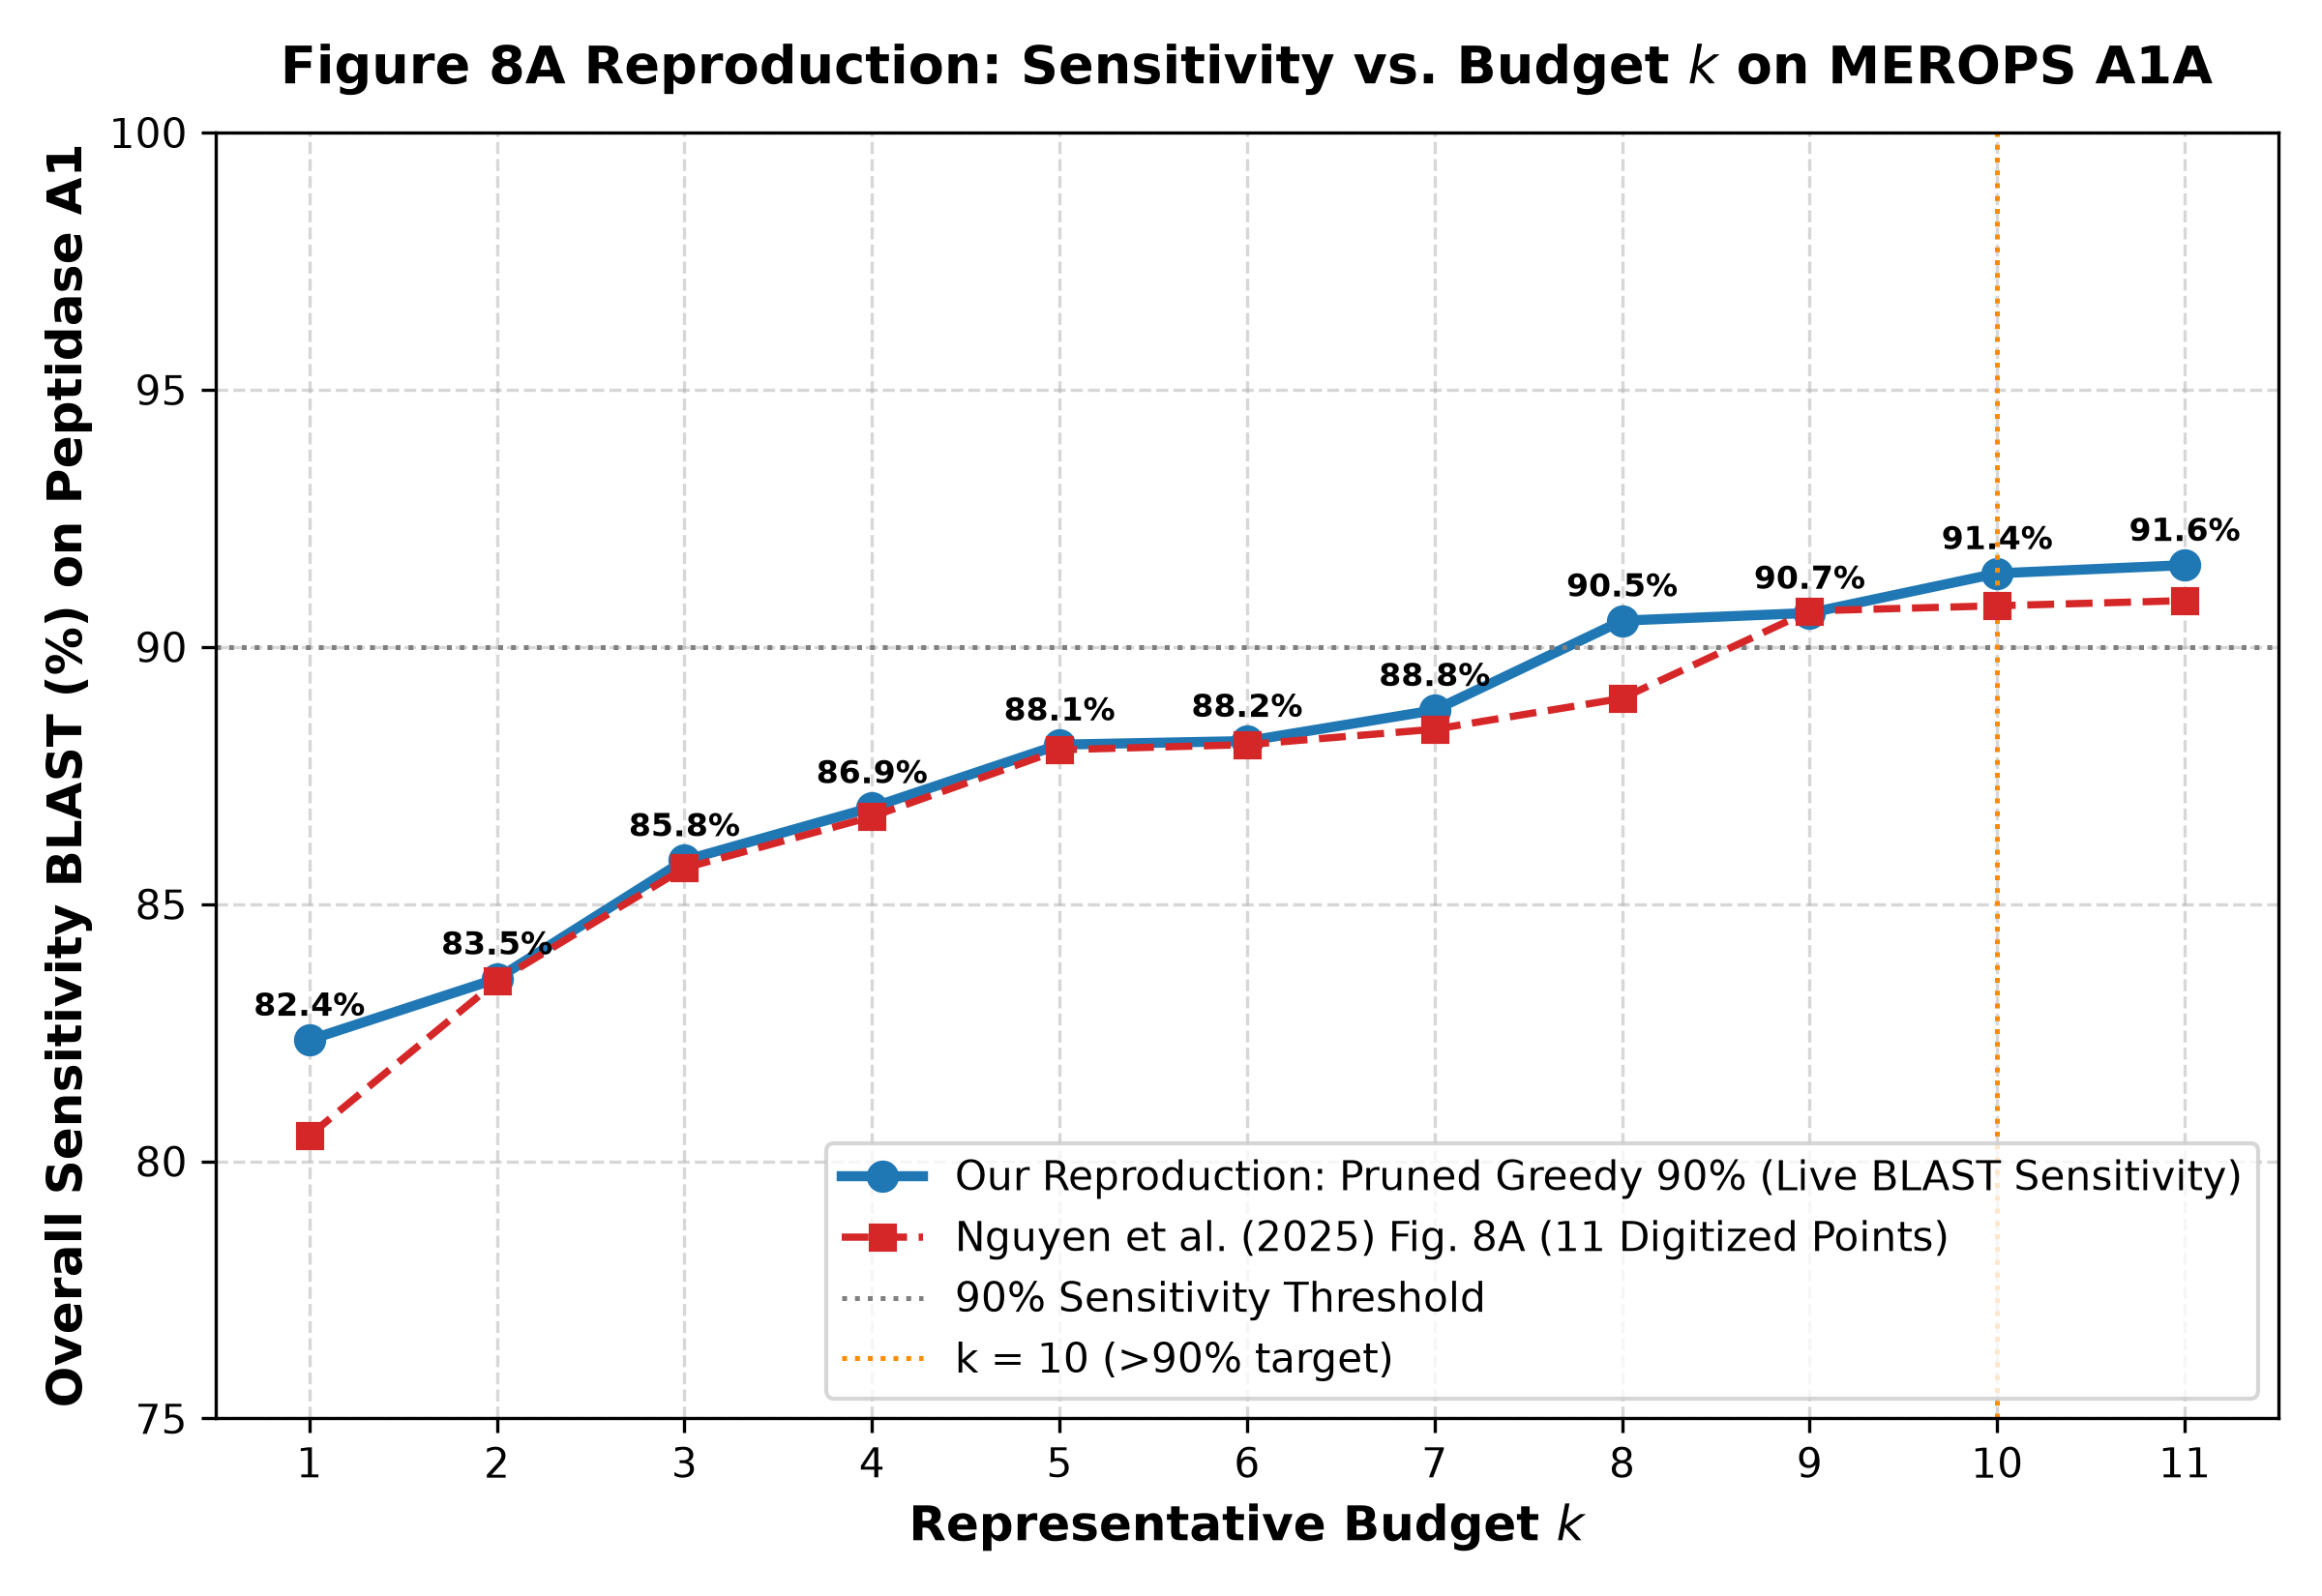
\includegraphics[width=0.84\textwidth]{Images/figures/exp1_a1a_sensitivity_vs_k.png}
    \caption{Đường cong Overall Sensitivity BLAST (\%) tái hiện trên Family Peptidase A1 đối chiếu với 11 điểm công bố tại hình 8A của Nguyen và cộng sự~\cite{nguyen2025}.}
    \label{fig:exp1_sensitivity}
\end{figure}

Số liệu tại bảng~\ref{tab:exp1_milestones} và hình~\ref{fig:exp1_sensitivity} khẳng định quy trình tái hiện thực nghiệm của đề tài đối chuẩn thành công công bố hình 8A của Nguyen và cộng sự~\cite{nguyen2025} với sai số tuyệt đối trung bình chỉ là $0{,}51\%$. Độ lệch giữa kết quả đo đạc thực nghiệm và dữ liệu công bố dao động trong biên độ hẹp từ $-0{,}04\%$ đến $+1{,}86\%$, tái hiện chuẩn xác xu thế tăng trưởng của chỉ số Overall Sensitivity khi vượt ngưỡng $90\%$ tại mốc ngân sách $k = 8$, đạt $90{,}51\%$ và nhận diện thành công $12.044$ trên $13.307$ chuỗi protein. Sự tương đồng định lượng này khẳng định thuật toán Pruned Greedy 90\% cùng ma trận tương đồng chuỗi $\mathbf{S}_{\text{BLAST}}$ đã tái lập chính xác mô hình cơ sở, tạo nền tảng vững chắc cho các thử nghiệm cải tiến tiếp theo.

Tuy nhiên, khi phân tích sâu cơ chế phân bổ ở cấp độ Subfamily, kết quả đối chứng làm sáng tỏ điểm mù phương pháp luận then chốt của mô hình không trọng số khi đánh giá toàn cục. Trong khi trên tập dữ liệu $13.307$ chuỗi thô, chỉ với một đại diện duy nhất ($k = 1$), chỉ số Overall Sensitivity đạt tới $82{,}36\%$ với $10.959$ chuỗi nhờ tích lũy bao phủ chéo sang các Subfamily khác và khối chuỗi chưa phân loại [A01.UPA], thì khi chuyển sang tập dữ liệu phân họ chính thức $V_{\text{curated}}$ gồm $4.120$ chuỗi với quy tắc đối soát nội phân họ Within-Subfamily, chỉ số Overall Sensitivity suy giảm mạnh: đại diện đầu tiên thuộc Subfamily lớn A01.001 chỉ thu hồi được $146 / 4.120$ chuỗi cùng Subfamily, tương ứng chỉ số Overall Sensitivity chỉ đạt $3{,}54\%$ và để lại $114$ trên $115$ Subfamily ở mức $0{,}0\%$ Sensitivity ($\text{Rare Sensitivity} = 0{,}0\%$, $\text{Macro-Average Sensitivity} = 0{,}87\%$). Tại mốc $k = 11$, chỉ số Overall Sensitivity nội phân họ của mô hình cơ sở không trọng số chỉ đạt $38{,}06\%$ với $1.568 / 4.120$ chuỗi và vẫn để sót $105$ trên $115$ Subfamily ở mức $0{,}0\%$. Kết quả thực nghiệm này làm rõ hạn chế cốt lõi của phương thức đánh giá toàn cục, chỉ ra rằng mức độ bao phủ trên $90\%$ ở bài báo gốc phần lớn được tạo thành từ hiện tượng bao phủ chéo ngoài ranh giới Subfamily.

\FloatBarrier
\phantomsection\label{sec:branch_2}
\phantomsection\label{subsec:branch2_mechanism}
\phantomsection\label{subsec:branch2_pareto}
\phantomsection\label{subsec:branch2_zero_cov}

Nhằm khắc phục điểm mù này, thử nghiệm 2 áp dụng nguyên tắc cô lập biến số: giữ nguyên không gian tương đồng chuỗi cơ sở NCBI BLASTp nhưng chuyển dịch sang tập dữ liệu phân họ chính thức $V_{\text{curated}}$ gồm $4.120$ chuỗi thuộc $115$ Subfamily, đồng thời đưa vào họ hàm mục tiêu có trọng số nghịch đảo quy mô Subfamily $w_v^{(\alpha)} = n_g^{-\alpha}$ với hệ số phạt quy mô nhóm $\alpha \in \{0{,}0, \, 0{,}5, \, 1{,}0\}$ đã định nghĩa tại công thức~\eqref{eq:sample_weight_formula}. Đồng thời, quy trình đo đạc áp dụng thống nhất cơ chế bao phủ nội phân họ Within-Subfamily Live BLASTp ở ngưỡng $E \le 10^{-7}$: chỉ các chuỗi đại diện thực sự thuộc về Subfamily $g$ mới được sử dụng làm chuỗi truy vấn đối soát với các thành viên của chính Subfamily đó, ngăn chặn nguy cơ sai lệch bao phủ chéo ngoài ranh giới phân họ.

Tại mốc ngân sách cơ sở $k = G = 115$, hàm mục tiêu có trọng số với $\alpha = 0{,}5$ đạt hiệu quả cao trên cả hai mục tiêu khi nâng chỉ số Rare Sensitivity tăng gấp $26{,}6$ lần, từ $2{,}22\%$ lên $59{,}11\%$, và chỉ số Macro-Average Sensitivity tăng thêm $+29{,}59\%$, từ $49{,}28\%$ lên $78{,}87\%$, trong khi chỉ số Overall Sensitivity không suy giảm mà tăng nhẹ từ $93{,}57\%$ lên $94{,}13\%$. Bảng~\ref{tab:exp2_milestones} tổng hợp kết quả tại các mốc ngân sách chiến lược.

\begin{table}[htbp!]
\centering
\caption{So sánh hiệu năng của ba chế độ trọng số $\alpha$ trên không gian tương đồng BLASTp tại các mốc ngân sách chiến lược theo cơ chế Within-Subfamily Live BLASTp.}
\label{tab:exp2_milestones}
\vspace{4pt}
\small
\resizebox{\textwidth}{!}{%
\begin{tabular}{ccrrrr}
\toprule
\textbf{Ngân sách $k$} & \textbf{Hệ số $\alpha$} & \textbf{Overall Sensitivity (\%)} & \textbf{Rare Sensitivity (\%)} & \textbf{Macro-Average Sensitivity (\%)} & \textbf{Zero-Sensitivity Count} \\
\midrule
$k = 15$  & 0{,}0 & 44{,}66 & 0{,}00  & 12{,}11 & 101 / 115 \\
          & 0{,}5 & 44{,}61 & 0{,}00  & 12{,}10 & 101 / 115 \\
          & 1{,}0 & 27{,}86 & 8{,}89  & 13{,}04 & 100 / 115 \\
\midrule
$k = 30$  & 0{,}0 & 71{,}65 & 0{,}00  & 23{,}87 & 87 / 115 \\
          & 0{,}5 & 62{,}72 & 4{,}44  & 25{,}15 & 86 / 115 \\
          & 1{,}0 & 48{,}16 & 26{,}67 & 26{,}03 & 85 / 115 \\
\midrule
$k = 60$  & 0{,}0 & 88{,}83 & 2{,}22  & 37{,}74 & 71 / 115 \\
          & 0{,}5 & 84{,}95 & 11{,}11 & 47{,}36 & 60 / 115 \\
          & 1{,}0 & 62{,}57 & 57{,}04 & 50{,}95 & 56 / 115 \\
\midrule
$k = 115$ & 0{,}0  & 93{,}57 & 2{,}22  & 49{,}28 & 58 / 115 \\
          & 0{,}5   & \textbf{94{,}13} & \textbf{59{,}11} & \textbf{78{,}87} & \textbf{23 / 115} \\
          & 1{,}0 & 79{,}08 & \textbf{91{,}11} & \textbf{83{,}44} & \textbf{18 / 115} \\
\bottomrule
\end{tabular}%
}
\end{table}

Số liệu tại bảng~\ref{tab:exp2_milestones} cho thấy sự cải thiện rõ nét khi áp dụng hàm mục tiêu có trọng số. Bên cạnh cấu hình trọng số cân bằng $\alpha = 0{,}5$, chế độ bình đẳng nhóm $\alpha = 1{,}0$ nâng chỉ số Rare Sensitivity lên mức cao nhất $91{,}11\%$, gấp $41{,}0$ lần so với mô hình cơ sở không trọng số, bảo tồn $41$ trên $45$ Subfamily hiếm nhưng chấp nhận sự đánh đổi khi chỉ số Overall Sensitivity giảm về $79{,}08\%$.

\begin{figure}[htbp!]
    \centering
    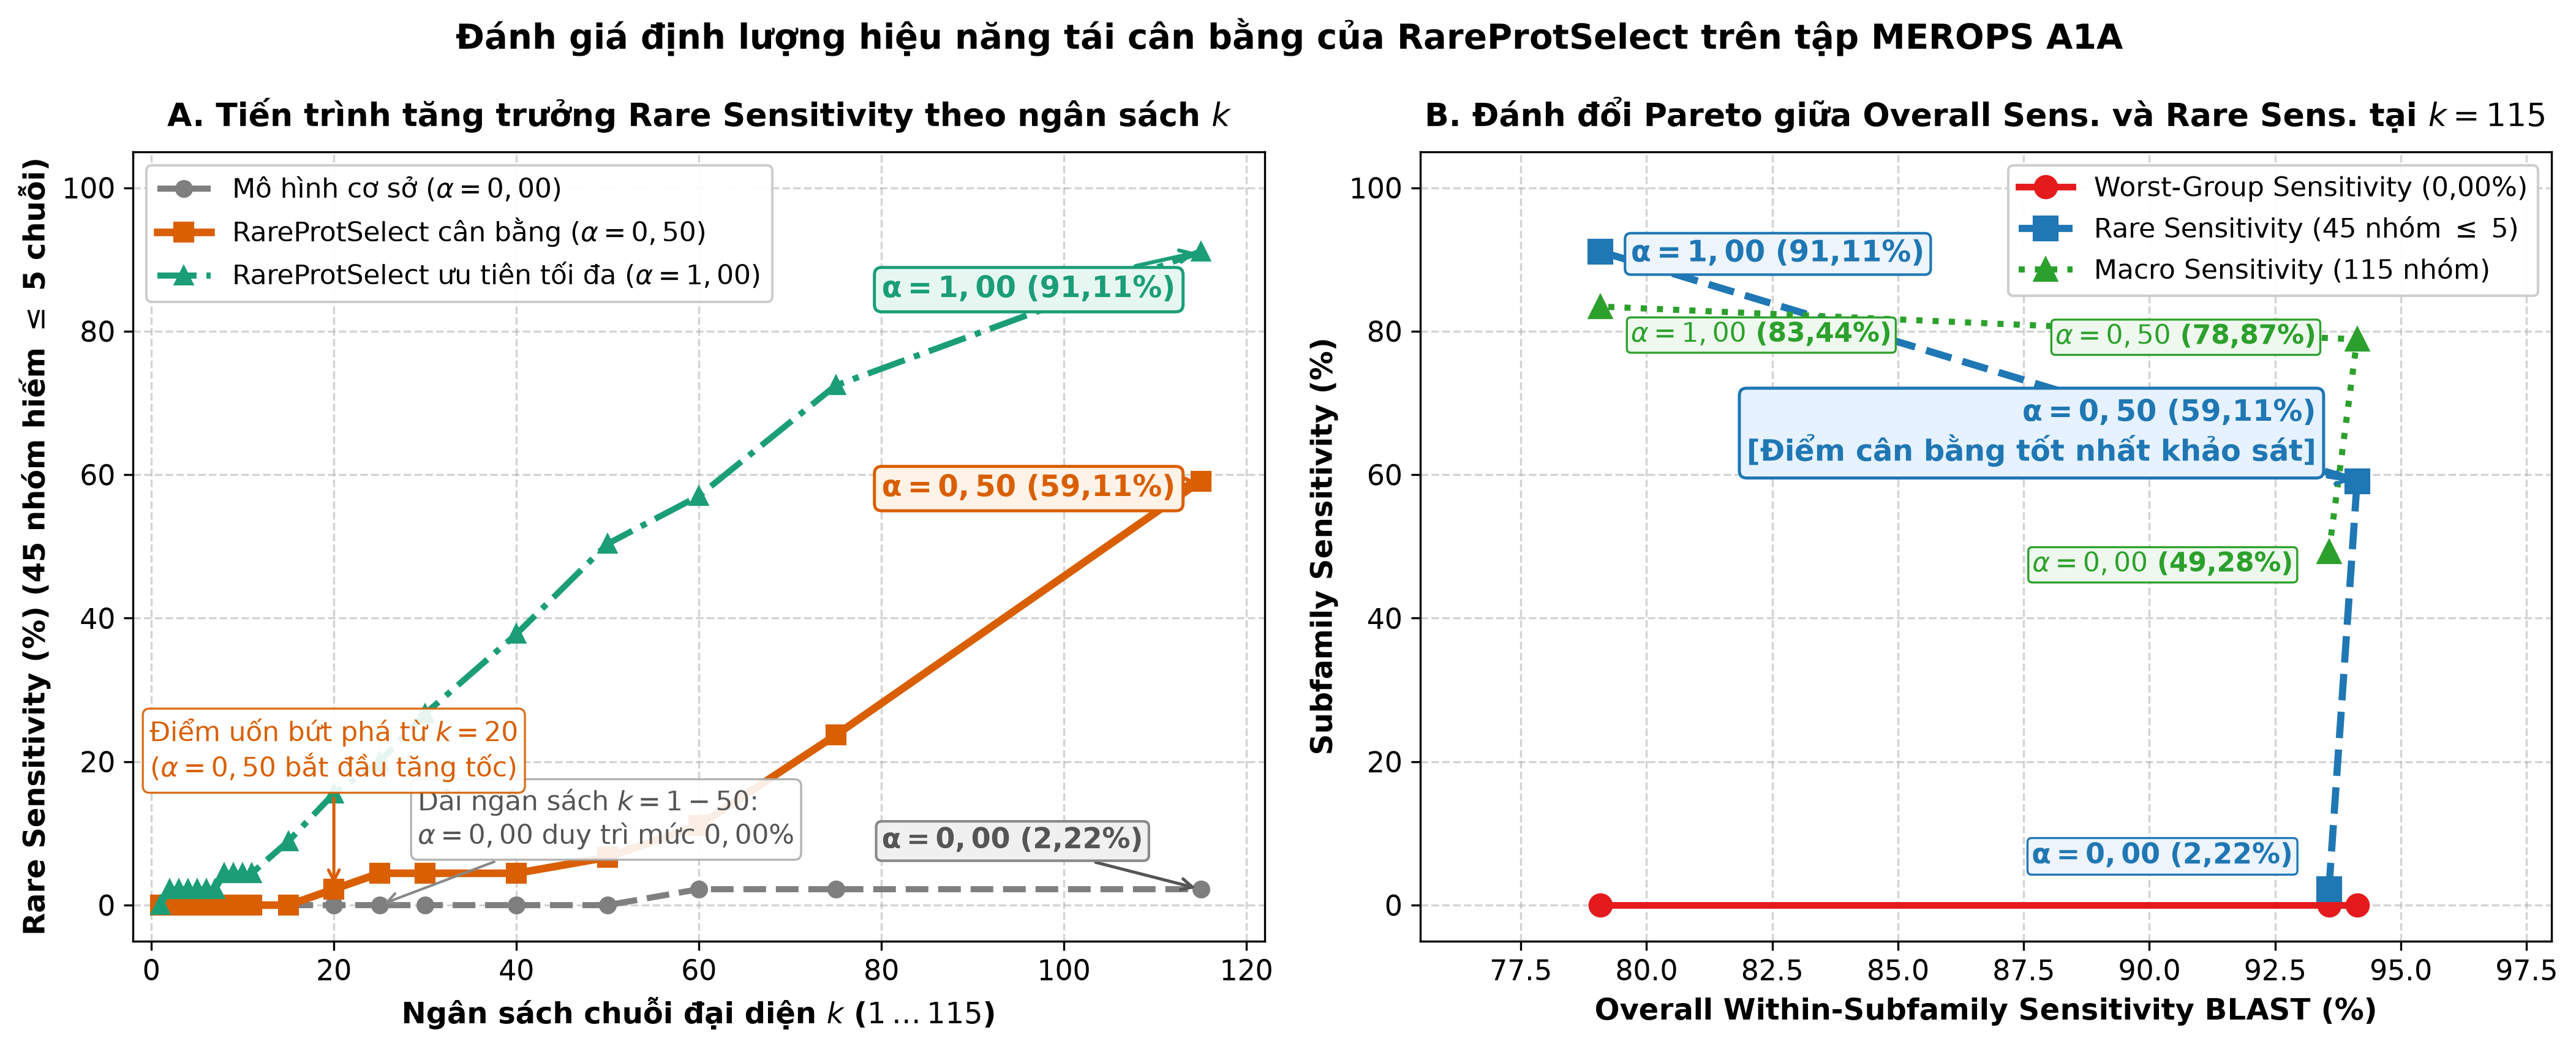
\includegraphics[width=0.92\textwidth]{Images/figures/exp2_pareto_tradeoff.png}
    \caption{Tương quan đánh đổi giữa chỉ số Overall Sensitivity và Rare Sensitivity tại hai mốc ngân sách $k = 11$ và $k = 115$ trên không gian tương đồng chuỗi BLASTp.}
    \label{fig:exp2_pareto}
\end{figure}

Mối quan hệ đánh đổi đa mục tiêu và xu hướng biến thiên của bốn chỉ số được minh họa tại hình~\ref{fig:exp2_pareto} và hình~\ref{fig:exp2_metrics}. Đồ thị làm rõ sự khác biệt giữa hai miền ngân sách: ở vùng ngân sách nhỏ $k = 11$ (hình~\ref{fig:exp2_pareto}A), sự đánh đổi đa mục tiêu thể hiện rõ khi $\alpha = 0{,}5$ có Overall Sensitivity đạt $32{,}60\%$ (thấp hơn $38{,}06\%$ của $\alpha = 0{,}0$) trong khi Rare Sensitivity vẫn bằng $0{,}0\%$ (chỉ có Macro-Average Sensitivity tăng nhẹ từ $8{,}68\%$ lên $9{,}56\%$); phải đến mốc ngân sách đủ lớn $k = G = 115$ (hình~\ref{fig:exp2_pareto}B), khi các Subfamily lớn đã đạt bão hòa nội nhóm, điểm biểu diễn của $\alpha = 0{,}5$ mới nằm ở góc trên bên phải so với $\alpha = 0{,}0$, nâng Rare Sensitivity lên $59{,}11\%$ mà không làm suy giảm Overall Sensitivity ($94{,}13\%$ so với $93{,}57\%$), trong khi $\alpha = 1{,}0$ tại $k = 115$ vẫn đánh đổi giảm $14{,}49$ điểm phần trăm Overall Sensitivity ($79{,}08\%$). Đồ thị hình~\ref{fig:exp2_metrics} thể hiện rõ sự chênh lệch giữa các chế độ trọng số: đường Rare Sensitivity của $\alpha = 0{,}0$ duy trì ở mức $0{,}0\%$ trong toàn bộ khoảng từ $k = 1$ đến $k = 50$, trong khi đường $\alpha = 1{,}0$ tăng trưởng nhanh ngay từ mốc $k = 2$ đạt $2{,}22\%$ và đạt $50{,}37\%$ tại mốc ngân sách $k = 50$. Đường Worst-Group Sensitivity (hình~\ref{fig:exp2_metrics}B) duy trì bằng $0{,}0\%$ xuyên suốt $k \in [1..115]$ do tại mọi mốc này vẫn còn ít nhất 18 Subfamily chưa có đại diện.

\begin{figure}[htbp!]
    \centering
    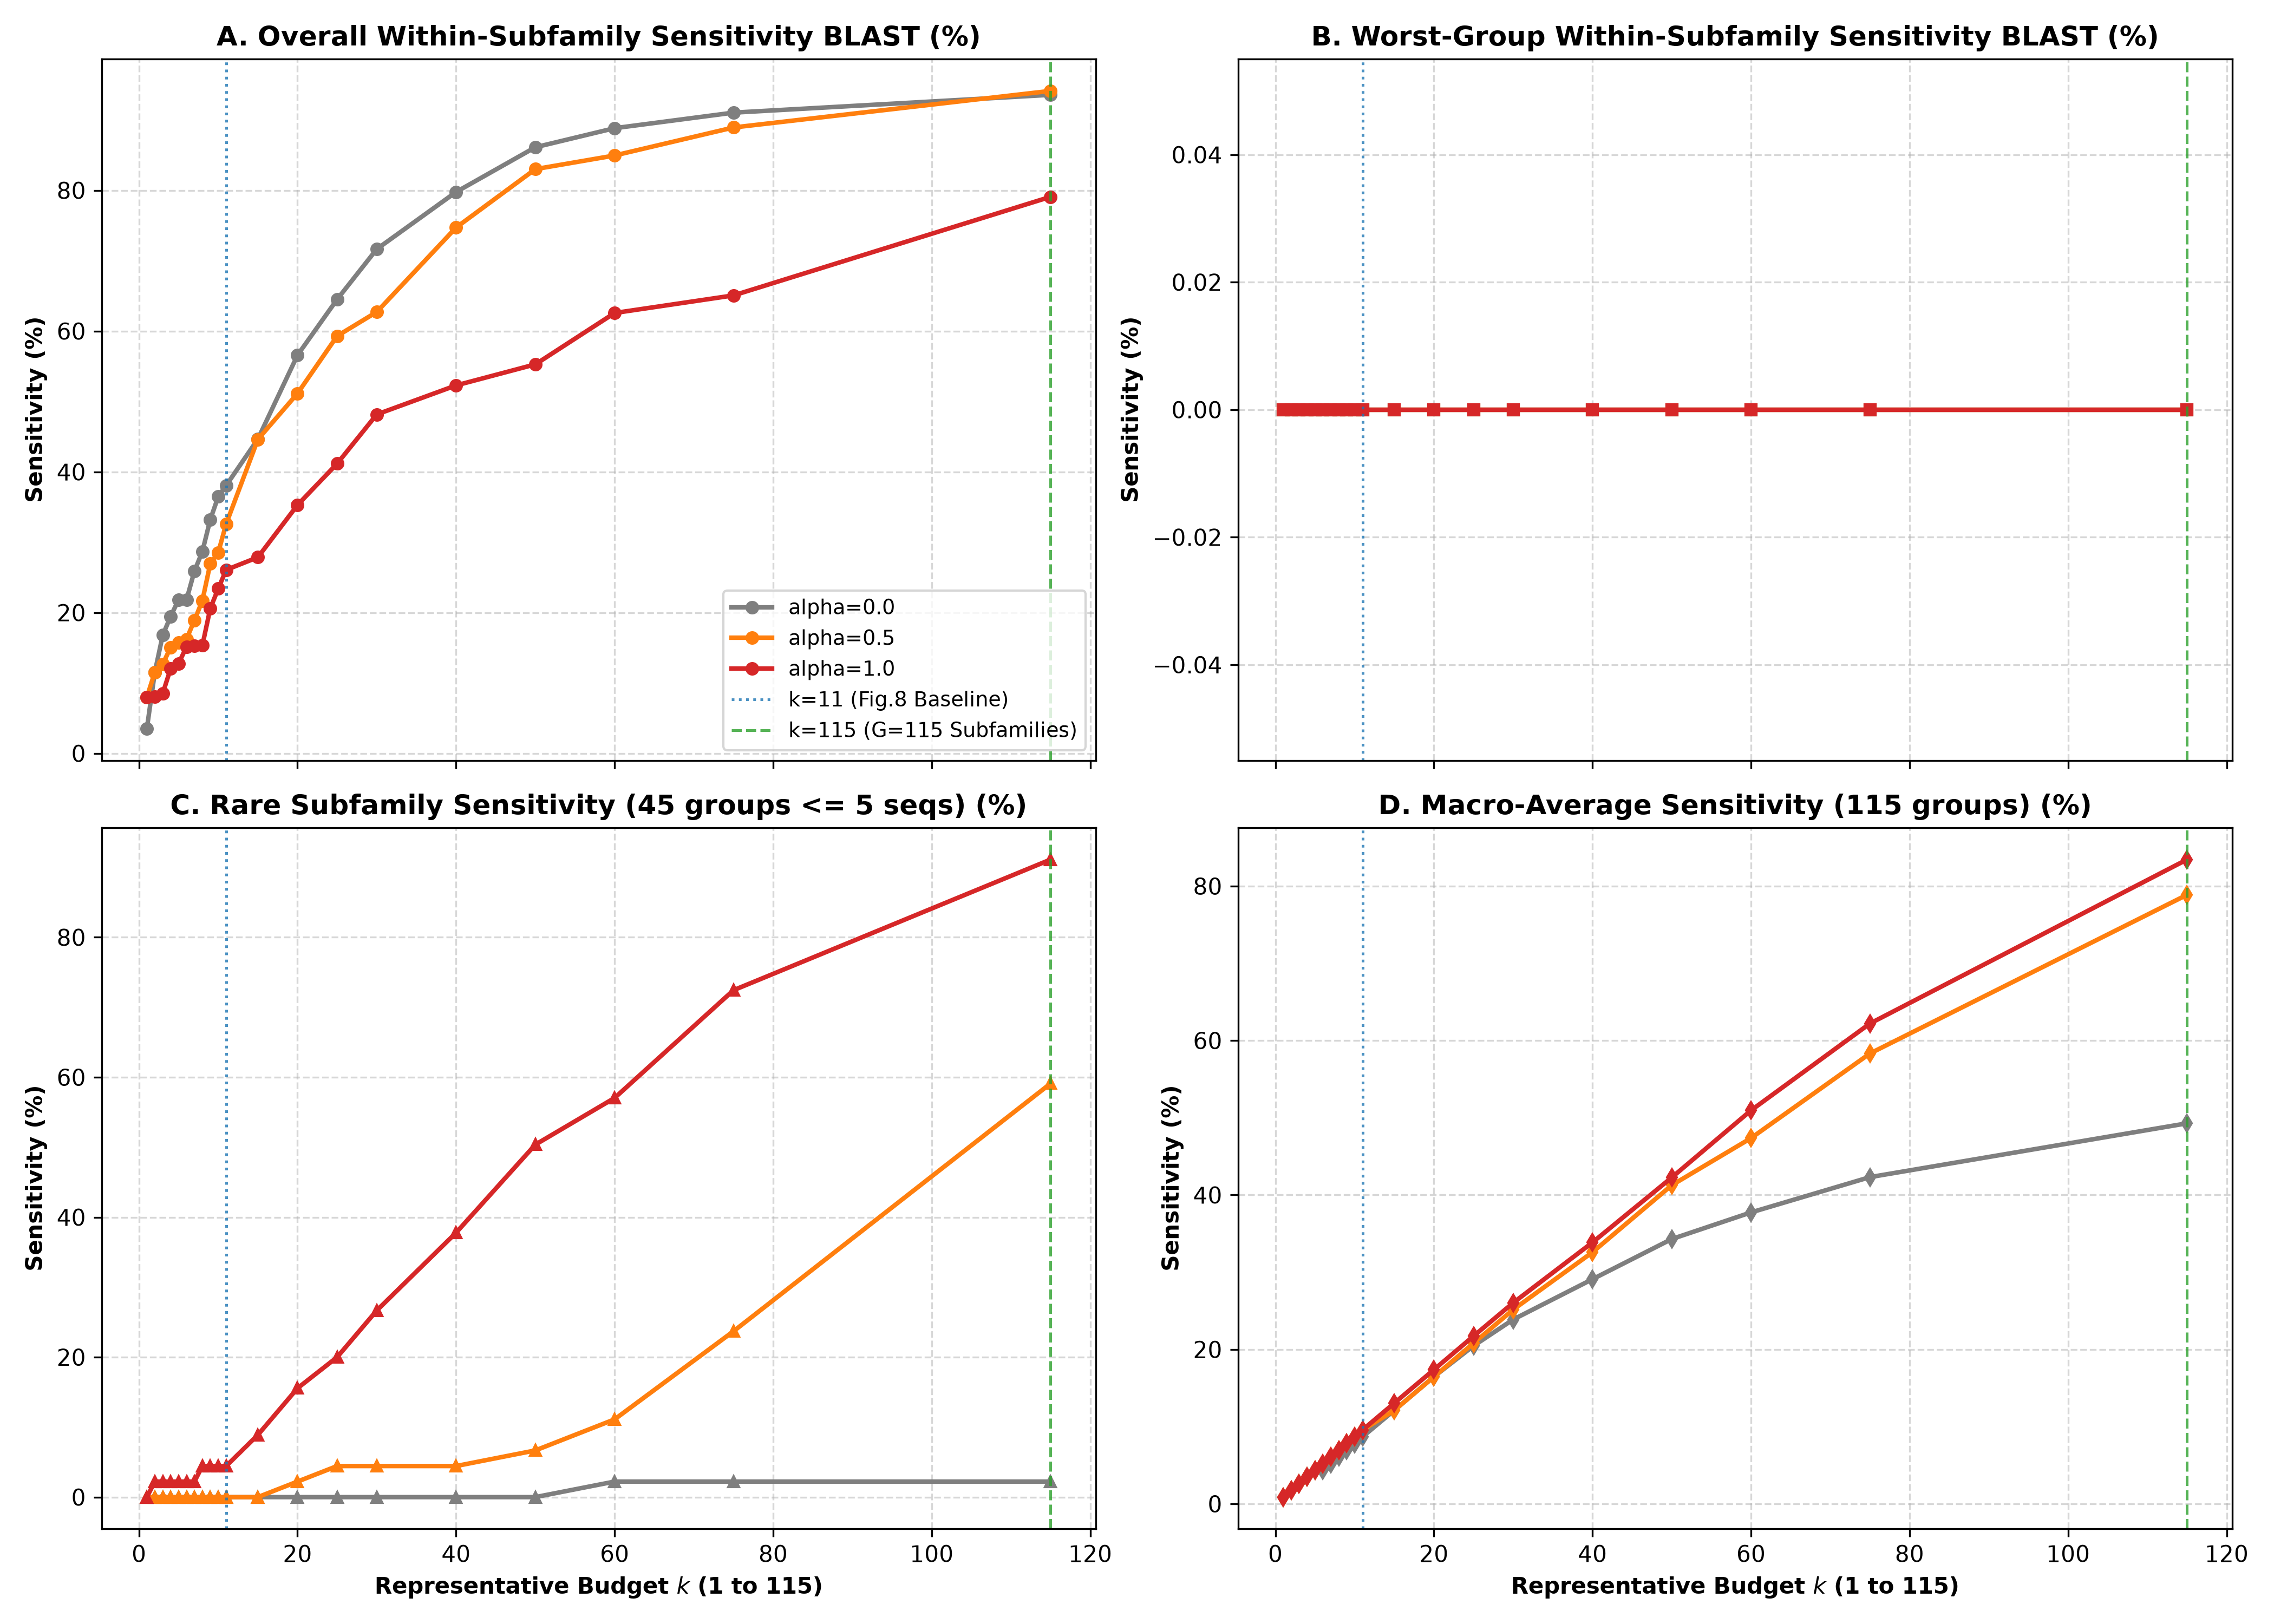
\includegraphics[width=0.92\textwidth]{Images/figures/exp2_metrics_vs_k.png}
    \caption{Đường cong biến thiên của bốn thước đo Sensitivity nội phân họ theo ngân sách $k \in [1..115]$ qua ba chế độ trọng số $\alpha \in \{0{,}0, \, 0{,}5, \, 1{,}0\}$ trên không gian BLASTp.}
    \label{fig:exp2_metrics}
\end{figure}

Thiết lập trọng số $\alpha = 0{,}5$ khôi phục tính đại diện cho $35$ Subfamily, kéo giảm số lượng phân họ có chỉ số Sensitivity bằng 0 từ $58$ xuống còn $23$ Subfamily tại mốc ngân sách $k = 115$. Hình~\ref{fig:exp2_zero_cov} lượng hóa số lượng phân họ có chỉ số Sensitivity bằng 0 theo hệ số $\alpha$, cho thấy phương pháp không trọng số của bài báo gốc để sót tới $58$ trên tổng số $115$ Subfamily, chiếm $50{,}43\%$, ở mức $0{,}0\%$ Sensitivity. Chế độ $\alpha = 1{,}0$ tiếp tục thu hẹp con số này về mức $18$ Subfamily. Kết quả này khẳng định hiệu quả của mô hình đề xuất: hàm mục tiêu có trọng số với $\alpha = 0{,}5$ khôi phục đáng kể tính đại diện cho các phân họ hiếm trên không gian BLASTp mà không làm giảm chỉ số Overall Sensitivity, nhờ cơ chế hạn chế các lượt chọn dư thừa ở các nhóm lớn.

\begin{figure}[htbp!]
    \centering
    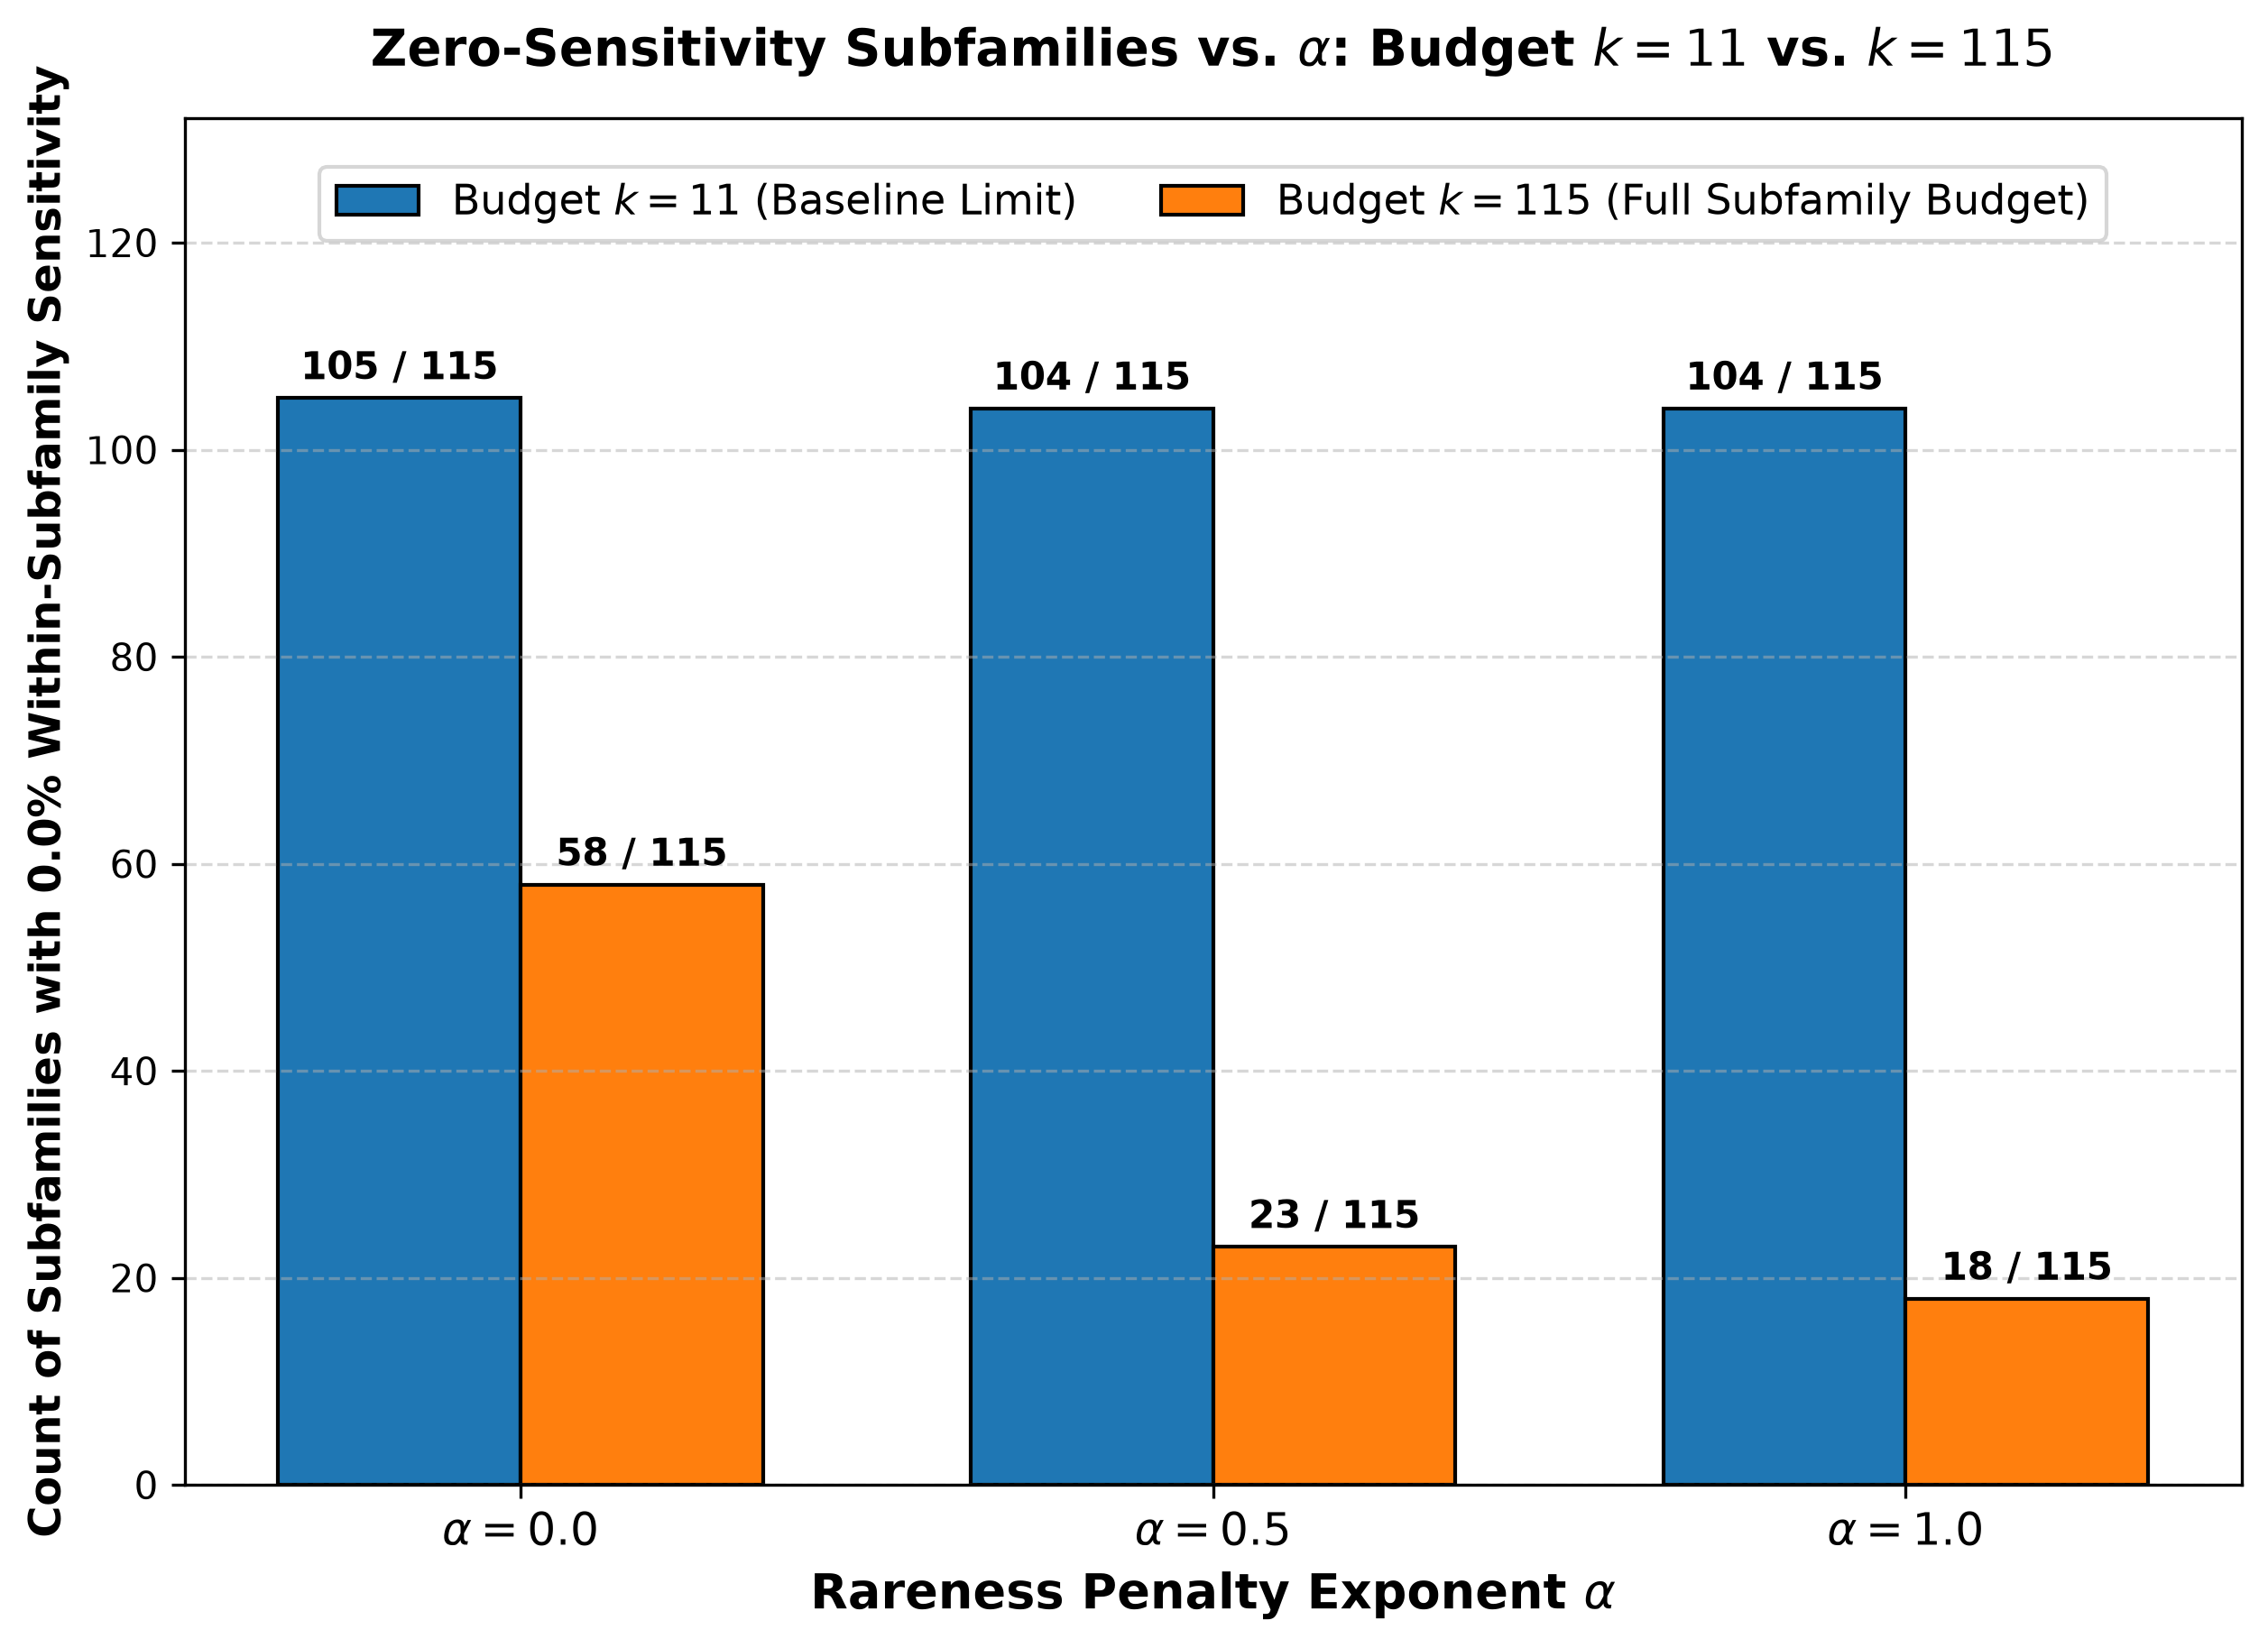
\includegraphics[width=0.82\textwidth]{Images/figures/exp2_zero_cov_vs_alpha.png}
    \caption{Biến thiên chỉ số Zero-Sensitivity Count theo hệ số $\alpha$ tại hai mốc ngân sách $k = 11$ và $k = 115$ trên không gian BLASTp.}
    \label{fig:exp2_zero_cov}
\end{figure}

\FloatBarrier\section{Khảo sát không gian ESM-2 và kiểm chứng chéo hai chiều}
\label{sec:esm_cross_evaluation}
\phantomsection\label{sec:branch_3}
\phantomsection\label{subsec:branch3_anisotropy}
\phantomsection\label{subsec:branch3_results}

Bên cạnh không gian tương đồng chuỗi rời rạc, hiệu năng bảo tồn đa dạng sinh học được khảo sát mở rộng trên không gian hình học liên tục ESM-2, kết hợp ma trận kiểm chứng chéo hai chiều nhằm đánh giá khả năng chuyển giao giữa hai hệ quy chiếu.

Tại thử nghiệm 3, giải thuật tối ưu hóa được thực thi trực tiếp trên ma trận tương đồng ngữ nghĩa $\mathbf{S}_{\text{ESM}}^{(\beta=0{,}70)}$ đã qua xử lý dịch tâm tại mục~\ref{subsec:mean_centering_technique} và đánh giá khả năng bao phủ cụm ngữ nghĩa bằng bốn thước đo hình học Within-Subfamily Coverage ESM. Trong không gian ngữ nghĩa liên tục, hàm mục tiêu có trọng số với $\alpha = 0{,}5$ nâng chỉ số Rare Coverage ESM tăng gấp $3{,}4$ lần, từ $12{,}85\%$ lên $43{,}21\%$, và chỉ số Macro-Average Coverage ESM tăng $+15{,}12\%$, từ $47{,}24\%$ lên $62{,}36\%$ tại ngân sách $k = 115$, trong khi chỉ số Overall Coverage ESM chỉ suy giảm nhẹ $-1{,}40\%$, từ $84{,}20\%$ xuống $82{,}80\%$. Bảng~\ref{tab:exp3_milestones} tổng hợp kết quả đo đạc qua ba chế độ trọng số tại các mốc ngân sách chiến lược.

\begin{table}[htbp!]
\centering
\caption{Hiệu năng bao phủ ngữ nghĩa nội phân họ Within-Subfamily Coverage ESM (\%) qua ba chế độ trọng số $\alpha$ tại các mốc ngân sách chiến lược.}
\label{tab:exp3_milestones}
\vspace{4pt}
\small
\resizebox{0.95\textwidth}{!}{%
\begin{tabular}{ccrrr}
\toprule
\textbf{Ngân sách $k$} & \textbf{Hệ số $\alpha$} & \textbf{Overall Coverage ESM (\%)} & \textbf{Rare Coverage ESM (\%)} & \textbf{Macro-Average Coverage ESM (\%)} \\
\midrule
$k = 8$   & 0{,}0 & 18{,}34 & 0{,}00  & 6{,}38 \\
          & 0{,}5 & 14{,}22 & \textbf{2{,}22}  & 6{,}37 \\
          & 1{,}0 & 14{,}42 & \textbf{2{,}22}  & 6{,}37 \\
\midrule
$k = 30$  & 0{,}0 & 59{,}73 & 2{,}05  & 22{,}94 \\
          & 0{,}5 & 52{,}75 & \textbf{10{,}86} & 23{,}32 \\
          & 1{,}0 & 31{,}78 & \textbf{28{,}26} & 23{,}69 \\
\midrule
$k = 60$  & 0{,}0 & 73{,}78 & 6{,}40  & 34{,}43 \\
          & 0{,}5 & 64{,}37 & \textbf{28{,}17} & 43{,}15 \\
          & 1{,}0 & 60{,}03 & \textbf{40{,}01} & 45{,}63 \\
\midrule
$k = 115$ & 0{,}0 & 84{,}20 & 12{,}85 & 47{,}24 \\
          & 0{,}5  & 82{,}80 & \textbf{43{,}21} & \textbf{62{,}36} \\
          & 1{,}0& 82{,}38 & \textbf{40{,}86} & 59{,}85 \\
\bottomrule
\end{tabular}%
}
\end{table}

Số liệu tại bảng~\ref{tab:exp3_milestones} cùng các đồ thị hình~\ref{fig:exp3_pareto} và hình~\ref{fig:exp3_metrics} khẳng định tính tổng quát của họ hàm mục tiêu có trọng số trong không gian hình học liên tục. Cần lưu ý rằng tại ngân sách nhỏ $k = 8$, ESM-2 ($\alpha = 0{,}5$) mới chọn được đúng $1 / 45$ Subfamily hiếm ($2{,}22\%$) và duy trì tỷ lệ này đến $k = 20$; trong khi trên không gian BLASTp, cấu hình $\alpha = 1{,}0$ đã chọn nhóm hiếm ngay từ $k = 2$ ($2{,}22\%$) và đạt $4{,}44\%$ tại $k = 8$. Lợi thế của ESM-2 ($\alpha = 0{,}5$) so với BLASTp ($\alpha = 0{,}5$) thể hiện rõ nhất ở dải ngân sách trung bình $k \in [25..60]$.

\begin{figure}[htbp!]
    \centering
    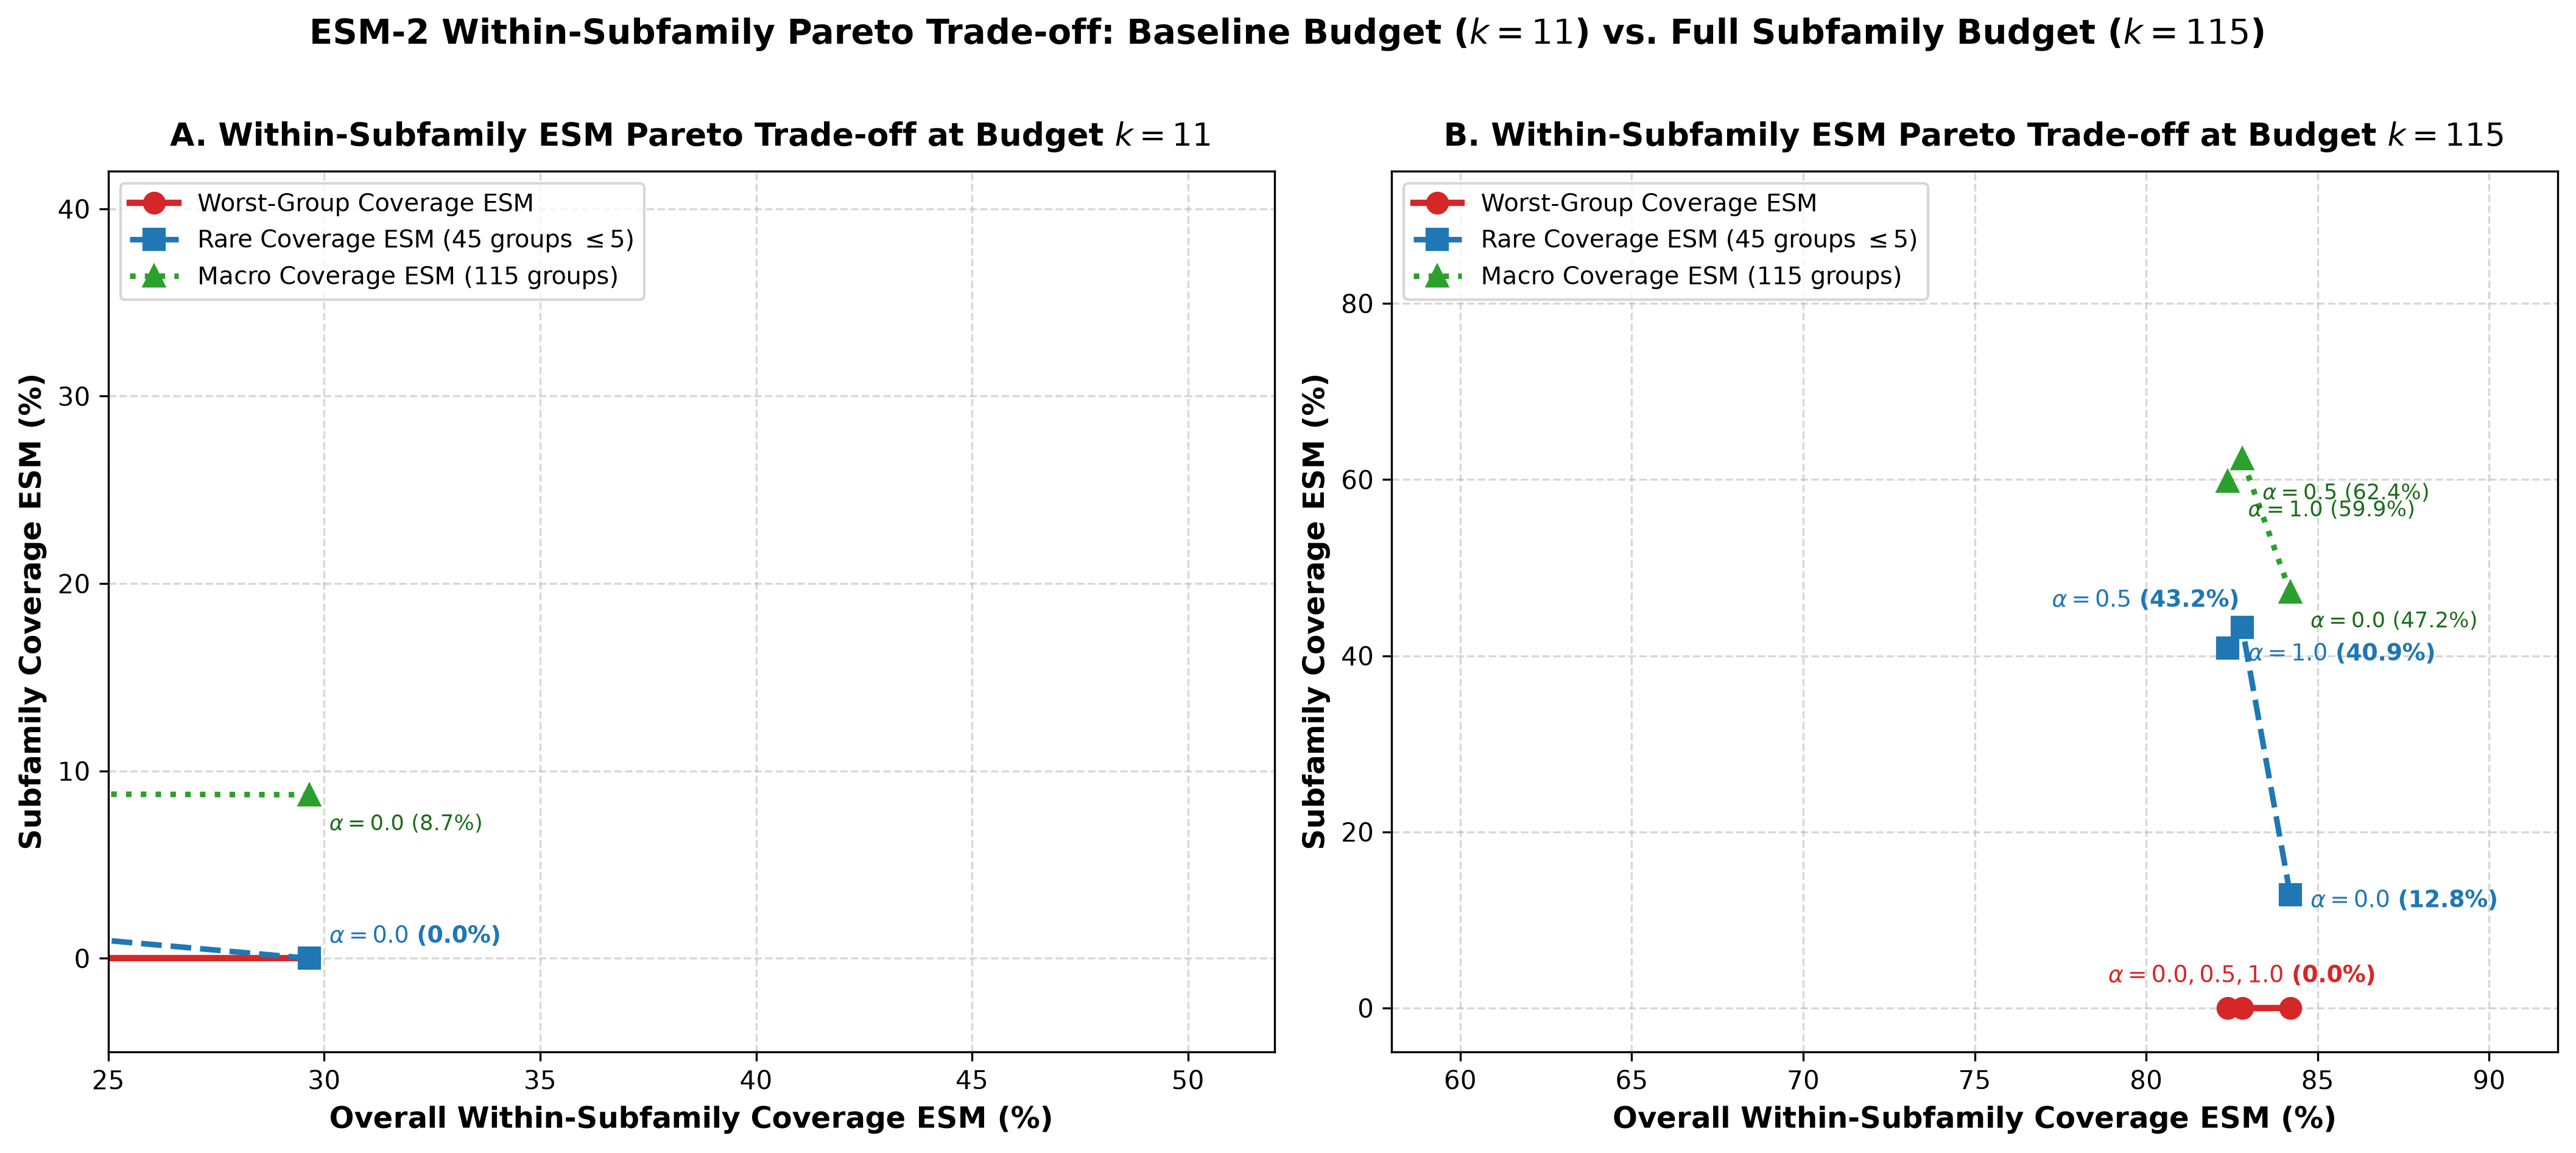
\includegraphics[width=0.92\textwidth]{Images/figures/exp3_pareto_tradeoff.png}
    \caption{Tương quan đánh đổi giữa Overall Coverage ESM và Rare Coverage ESM tại hai mốc ngân sách $k = 11$ và $k = 115$ trên không gian ngữ nghĩa ESM-2.}
    \label{fig:exp3_pareto}
\end{figure}

\begin{figure}[htbp!]
    \centering
    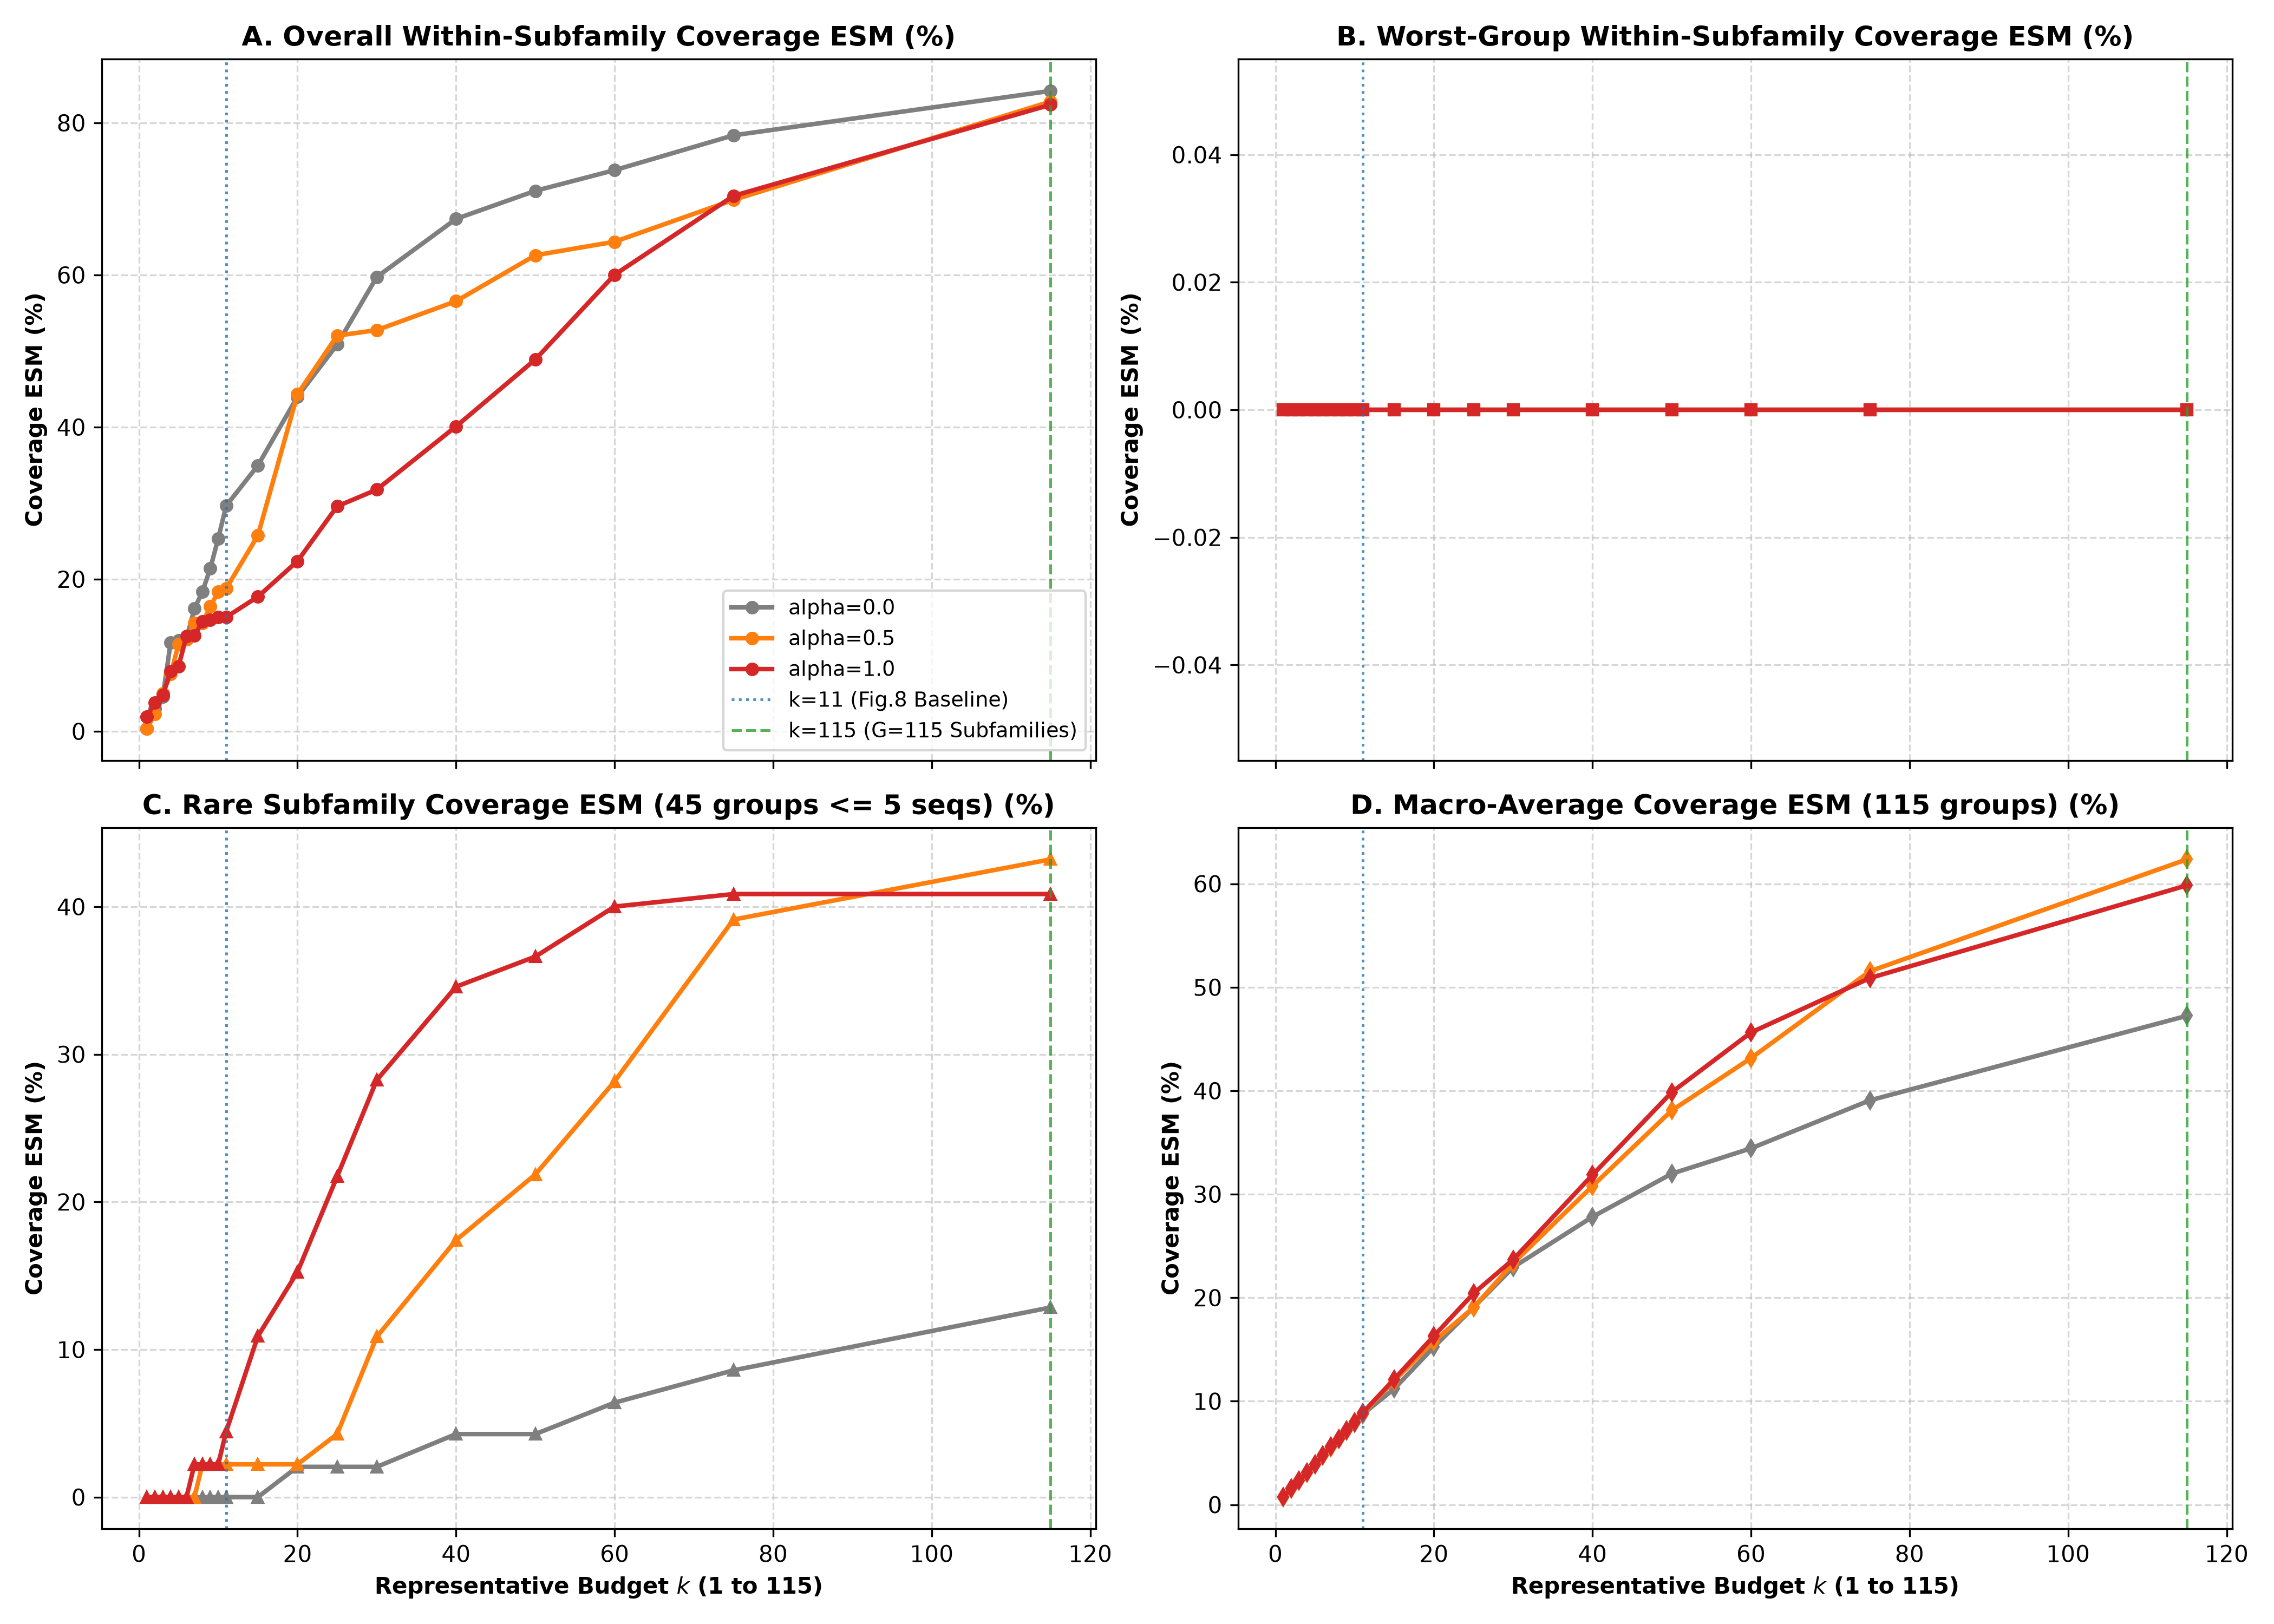
\includegraphics[width=0.92\textwidth]{Images/figures/exp3_metrics_vs_k.png}
    \caption{Đường cong biến thiên của bốn chỉ số Within-Subfamily Coverage ESM (\%) theo ngân sách $k \in [1..115]$ qua ba chế độ trọng số $\alpha$ trên không gian ESM-2.}
    \label{fig:exp3_metrics}
\end{figure}

\FloatBarrier
\phantomsection\label{sec:branch_4}
\phantomsection\label{subsec:branch4_matrix_design}
\phantomsection\label{subsec:branch4_crossover}
\phantomsection\label{subsec:branch4_math_explanation}

Nhằm kiểm soát hiện tượng thiên lệch khi đánh giá nội không gian, thử nghiệm 4 triển khai ma trận kiểm chứng chéo hai chiều $2 \times 2$ trên toàn bộ $120$ cấu hình thực nghiệm đối với cả hai hệ quy chiếu: thước đo sinh học thực nghiệm Within-Subfamily Live BLASTp ở ngưỡng $E \le 10^{-7}$ và thước đo hình học bổ trợ Within-Subfamily Coverage ESM trên ma trận $\mathbf{S}_{\text{ESM}}^{(\beta=0{,}70)}$. Toàn bộ $60$ cấu hình đường chéo chính khớp $100{,}00\%$ khi đối chiếu với kết quả gốc của thử nghiệm 2 và thử nghiệm 3.

Kiểm tra chéo hai chiều cho thấy sự đảo chiều về hiệu năng giữa hai không gian khi tăng ngân sách $k$: ở dải ngân sách nhỏ và vừa từ $k = 8$ đến $k = 75$, tập đại diện chọn bởi ESM-2 đạt kết quả cao hơn so với BLASTp, gấp từ $1{,}6$ lần đến $4{,}0$ lần; tuy nhiên, khi ngân sách tăng lên $k = 115$, tập đại diện chọn bởi BLASTp lại đạt kết quả cao hơn trên cả hai hệ quy chiếu đo đạc. Bảng~\ref{tab:exp4_cross_milestones} tổng hợp kết quả đối sánh hai chiều tại các mốc ngân sách khảo sát.

\begin{table}[htbp!]
\centering
\caption{Đối chiếu kiểm tra chéo hai chiều giữa đại diện chọn bởi BLASTp và đại diện chọn bởi ESM-2 trên cả hai hệ quy chiếu đo đạc tại các mốc ngân sách khảo sát.}
\label{tab:exp4_cross_milestones}
\vspace{4pt}
\small
\resizebox{\textwidth}{!}{%
\begin{tabular}{cccrrrr}
\toprule
\textbf{Không gian chọn} & \textbf{Hệ số $\alpha$} & \textbf{Ngân sách $k$} & \textbf{Overall Sensitivity (\%)} & \textbf{Rare Sensitivity (\%)} & \textbf{Overall Coverage ESM (\%)} & \textbf{Rare Coverage ESM (\%)} \\
\midrule
BLASTp & 0{,}0 & $k = 115$ & 93{,}57 & 2{,}22  & 87{,}47 & 2{,}05 \\
ESM-2  & 0{,}0 & $k = 115$ & 90{,}70 & \textbf{13{,}33} & 84{,}20 & \textbf{12{,}85} \\
\midrule
BLASTp & 0{,}5 & $k = 40$  & 74{,}71 & 4{,}44  & 68{,}71 & 4{,}27 \\
ESM-2  & 0{,}5 & $k = 40$  & 59{,}85 & \textbf{17{,}78} & 56{,}55 & \textbf{17{,}41} \\
\midrule
BLASTp & 0{,}5 & $k = 60$  & 84{,}95 & 11{,}11 & 77{,}91 & 10{,}83 \\
ESM-2  & 0{,}5 & $k = 60$  & 67{,}91 & \textbf{28{,}89} & 64{,}37 & \textbf{28{,}17} \\
\midrule
BLASTp & 0{,}5 & $k = 115$ & \textbf{94{,}13} & \textbf{59{,}11} & \textbf{86{,}88} & \textbf{58{,}29} \\
ESM-2  & 0{,}5 & $k = 115$ & 89{,}98 & 43{,}11 & 82{,}80 & 43{,}21 \\
\midrule
BLASTp & 1{,}0 & $k = 115$ & 79{,}08 & \textbf{91{,}11} & 72{,}75 & \textbf{89{,}69} \\
ESM-2  & 1{,}0 & $k = 115$ & 87{,}79 & 41{,}33 & 82{,}38 & 40{,}86 \\
\bottomrule
\end{tabular}%
}
\end{table}

\begin{figure}[htbp!]
    \centering
    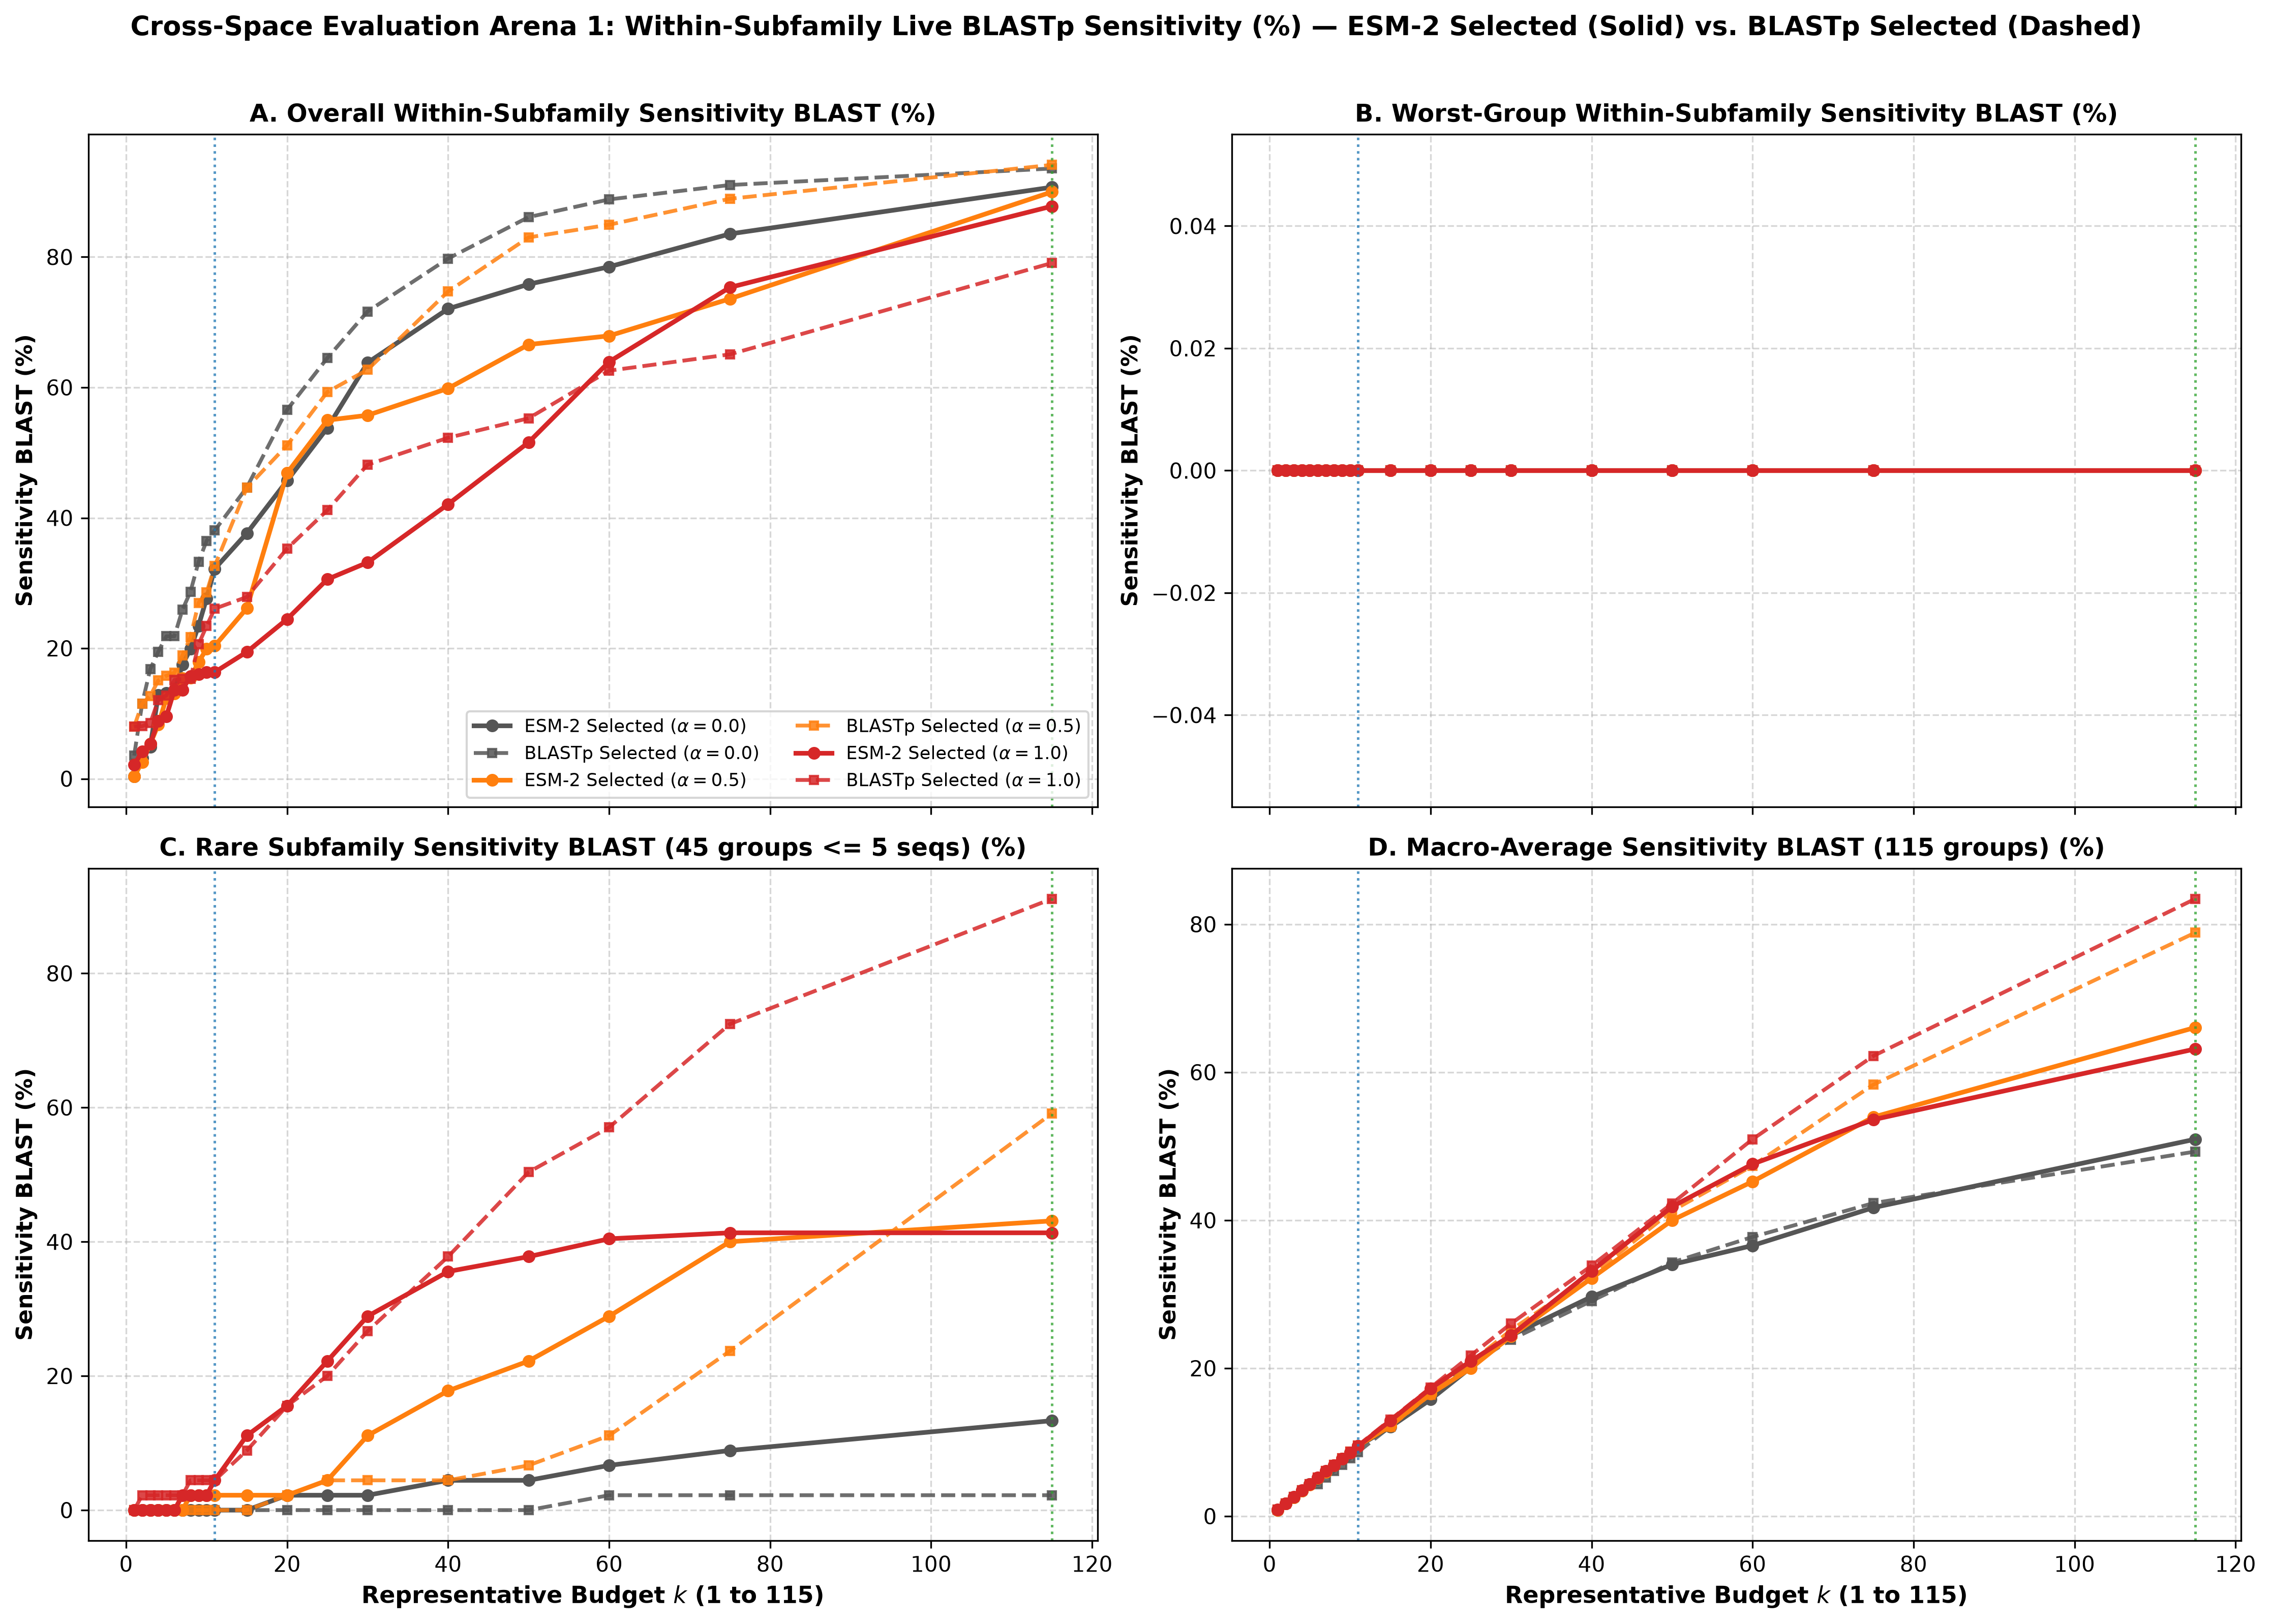
\includegraphics[width=0.92\textwidth]{Images/figures/exp4_blast_eval_comparison_vs_k.png}
    \caption{Hệ quy chiếu thứ nhất: so sánh hiệu năng giữa đại diện chọn bởi ESM-2 biểu diễn bằng đường nét liền và đại diện chọn bởi BLASTp biểu diễn bằng đường nét đứt trên thước đo Within-Subfamily Live BLASTp Sensitivity (\%) theo ngân sách $k \in [1..115]$.}
    \label{fig:exp4_blast_eval}
\end{figure}

\begin{figure}[htbp!]
    \centering
    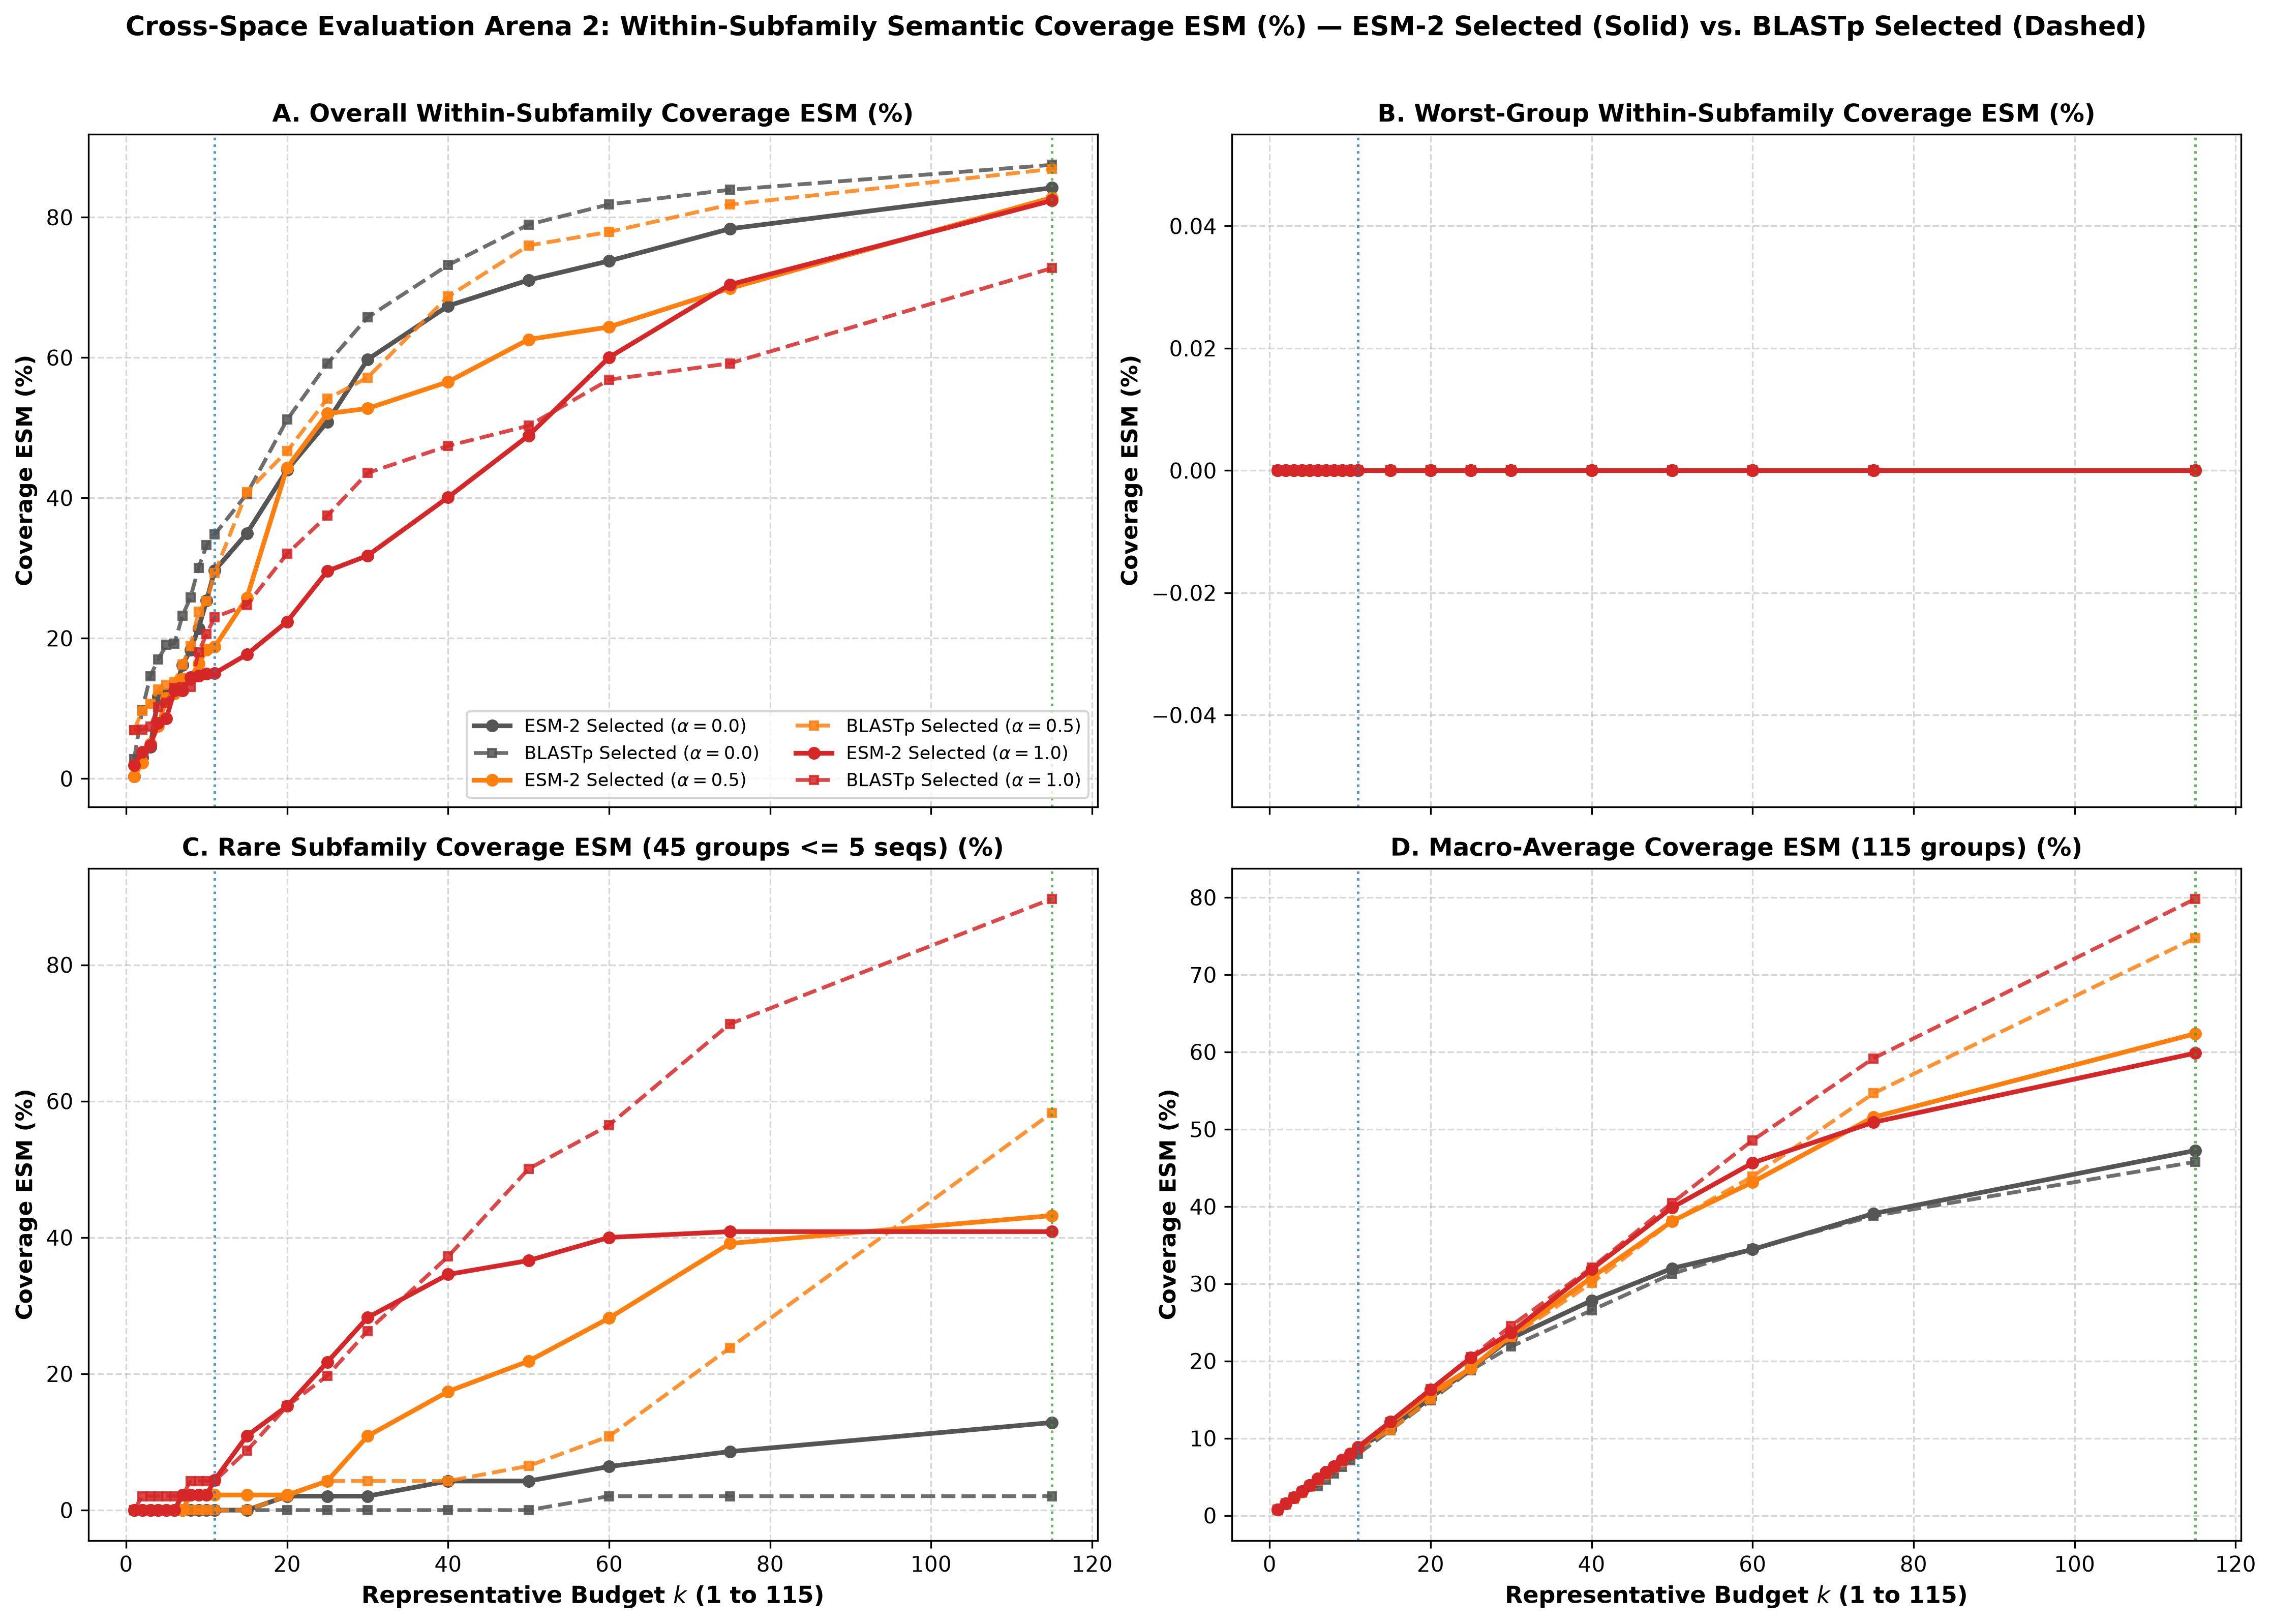
\includegraphics[width=0.92\textwidth]{Images/figures/exp4_esm_eval_comparison_vs_k.png}
    \caption{Hệ quy chiếu thứ hai: so sánh hiệu năng giữa đại diện chọn bởi ESM-2 biểu diễn bằng đường nét liền và đại diện chọn bởi BLASTp biểu diễn bằng đường nét đứt trên thước đo Within-Subfamily Coverage ESM (\%) theo ngân sách $k \in [1..115]$.}
    \label{fig:exp4_esm_eval}
\end{figure}

\FloatBarrier
Nguyên nhân toán học của sự đảo chiều về hiệu năng giữa hai không gian tại hình~\ref{fig:exp4_blast_eval}, hình~\ref{fig:exp4_esm_eval} và hình~\ref{fig:exp4_summary} bắt nguồn từ sự khác biệt cấu trúc giữa ma trận đặc ESM-2 và ma trận thưa BLASTp. Ma trận ngữ nghĩa $\mathbf{S}_{\text{ESM}}$ là ma trận đặc với $99{,}64\%$ cặp phần tử mang giá trị dương, giúp mỗi đại diện được chọn ở giai đoạn đầu ($k \le 75$) lan tỏa độ bao phủ sang các cụm lân cận và nhận diện sớm nhiều nhóm hiếm. Tuy nhiên, khi ngân sách tiến dần về $k = 115$, do mức tương đồng nền đã cao sẵn, phần độ tăng cận biên còn lại của các Subfamily hiếm bị thu hẹp và nhỏ hơn tổng độ tăng cận biên tích lũy trên hàng trăm chuỗi của các Subfamily lớn, khiến giải thuật ưu tiên chọn thêm đại diện cho nhóm lớn. Ngược lại, ma trận $\mathbf{S}_{\text{BLAST}}$ là ma trận thưa với độ tương đồng giữa các Subfamily xa nhau bằng $0{,}0$; khi các nhóm lớn đã được bao phủ nội bộ ở cuối dải ngân sách, độ tăng cận biên của chúng giảm về gần $0$, giúp các Subfamily hiếm chưa có đại diện giữ được độ tăng cận biên cao hơn và lần lượt được lựa chọn. Đặc biệt, tại mốc ngân sách trung bình $k = 60$, cấu hình BLASTp với trọng số mạnh $\alpha = 1{,}0$ đạt Rare Sensitivity lên tới $57{,}04\%$ và Overall Sensitivity đạt $62{,}57\%$, cao hơn so với ESM-2 $\alpha = 0{,}5$ ($28{,}89\%$ Rare Sensitivity, $67{,}91\%$ Overall Sensitivity) và ESM-2 $\alpha = 1{,}0$ ($40{,}44\%$ Rare Sensitivity, $63{,}93\%$ Overall Sensitivity). Như vậy, kiểm chứng chéo hai chiều cho thấy trọng số $\alpha = 0{,}5$ cải thiện tỷ lệ nhận diện nhóm hiếm trên cả hai không gian; trong đó không gian ESM-2 phát huy ưu thế bao phủ cụm ngữ nghĩa ở ngân sách vừa, còn không gian BLASTp với $\alpha \in \{0{,}5, 1{,}0\}$ bao phủ các phân họ hiếm đầy đủ hơn khi xét trên thước đo nhận diện chuỗi thực nghiệm Live BLASTp.

\begin{figure}[htbp!]
    \centering
    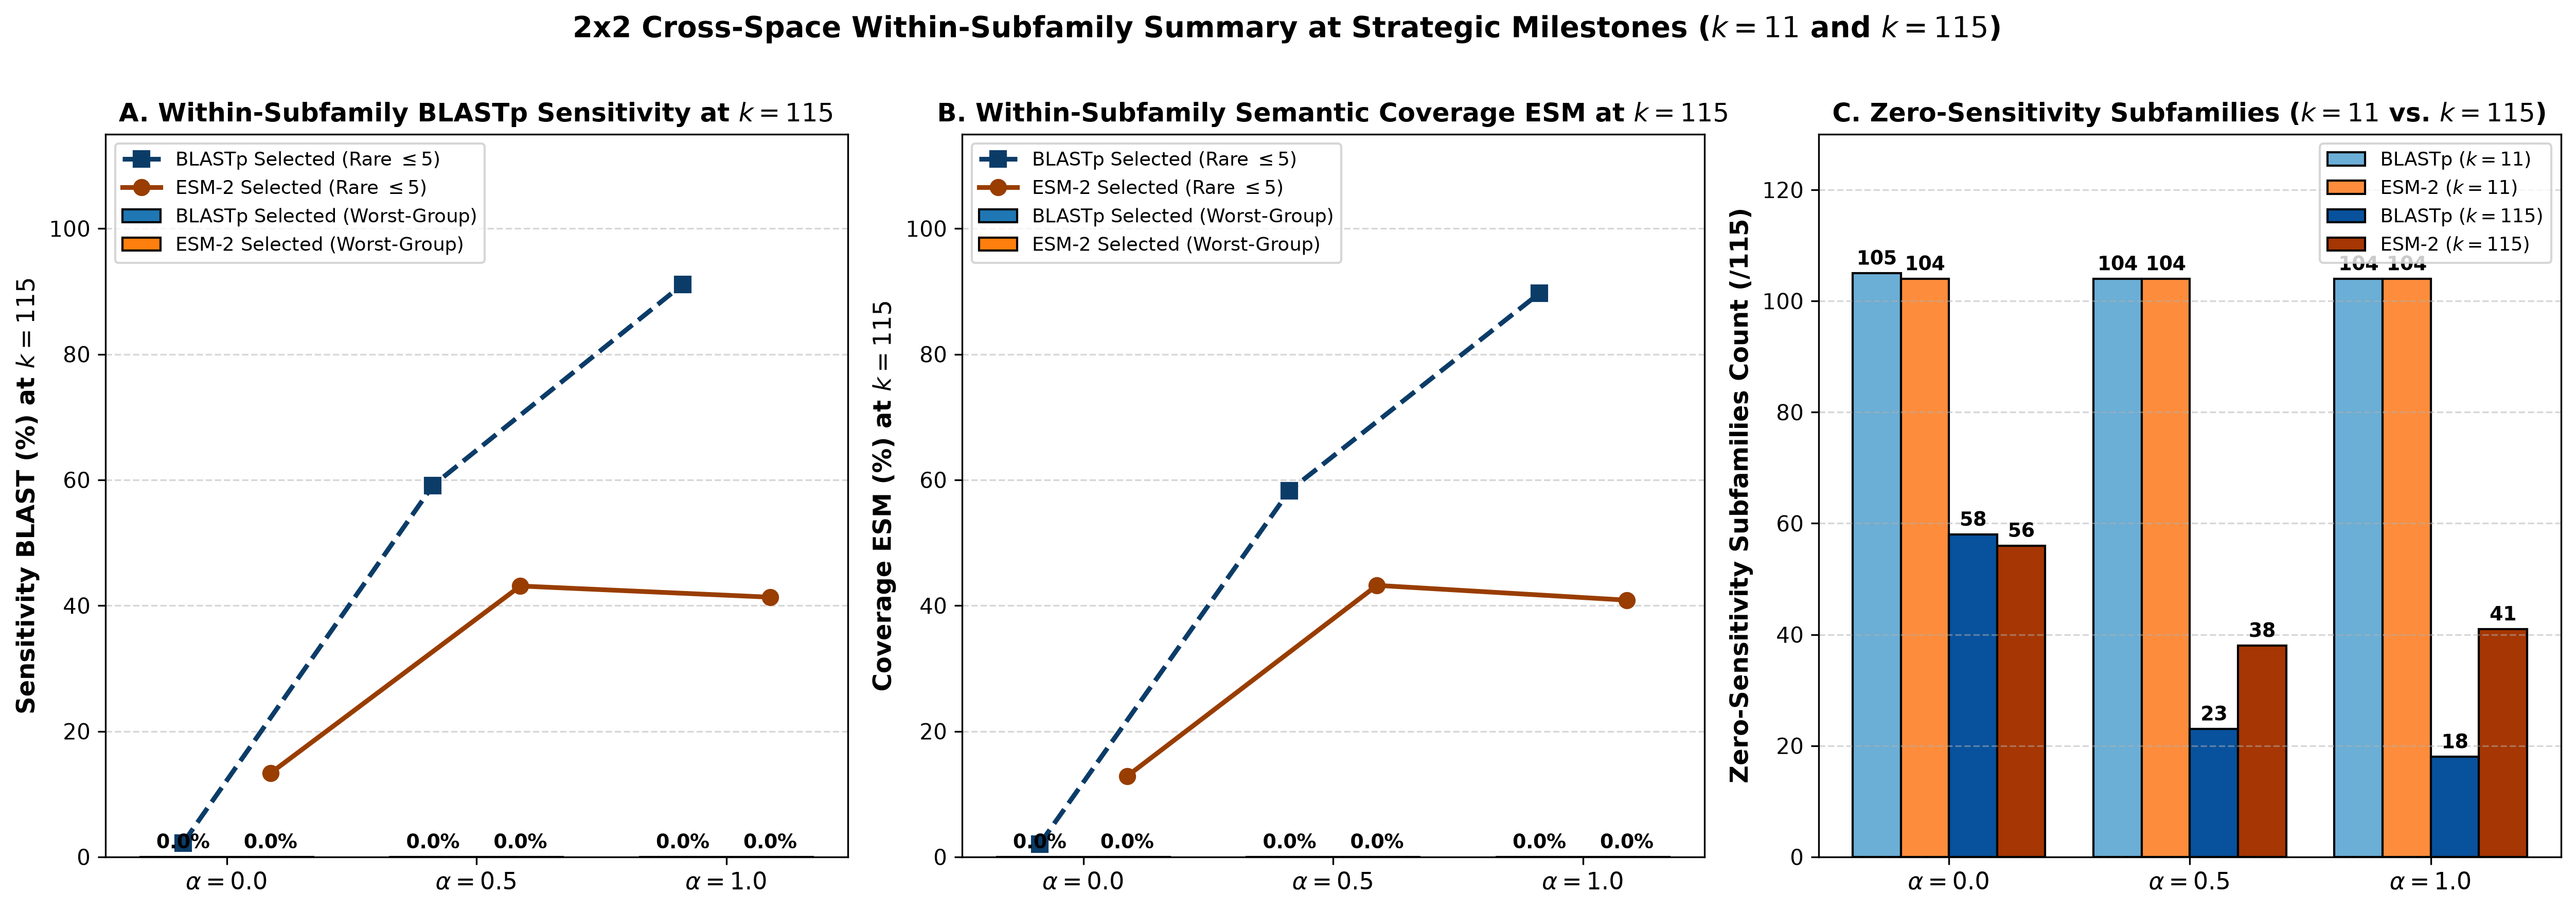
\includegraphics[width=0.92\textwidth]{Images/figures/exp4_cross_space_summary_k11_k76.png}
    \caption{Biểu đồ tổng hợp đối chiếu chéo hai chiều giữa đại diện chọn bởi BLASTp và đại diện chọn bởi ESM-2 tại hai mốc chiến lược $k = 11$ và $k = 115$.}
    \label{fig:exp4_summary}
\end{figure}

\FloatBarrier\section{Phân tích cơ chế phân bổ đại diện và khảo sát độ bão hòa khi mở rộng ngân sách}
\label{sec:allocation_saturation_discussion}
\phantomsection\label{sec:branch_5}
\phantomsection\label{subsec:branch5_invariants}
\phantomsection\label{subsec:branch5_results}

Nhằm làm rõ cơ chế vi mô giúp hàm mục tiêu có trọng số cải thiện đáng kể tỷ lệ nhận diện các phân họ hiếm mà không làm suy giảm độ bao phủ tổng thể, thử nghiệm 5 phân tích trực tiếp cơ cấu nhãn Subfamily của từng chuỗi đại diện bên trong tập nghiệm $S_k$ trên toàn bộ $120$ cấu hình thực nghiệm.

Kết quả phân tích chỉ ra rằng tại ngân sách $k = 115$, mô hình không trọng số ($\alpha = 0{,}0$) phân bổ lặp lại tới $58$ vị trí đại diện vào các Subfamily lớn đã có đại diện, đẩy chỉ số dư thừa phân bổ Subfamily Redundancy lên mức $50{,}43\%$ và khiến $58$ trên $115$ Subfamily không có đại diện. Ngược lại, tại cùng mốc ngân sách $k = 115$, RareProtSelect với trọng số $\alpha = 0{,}5$ giảm đáng kể độ dư thừa phân bổ từ $50{,}43\%$ xuống còn $20{,}00\%$, chuyển $35$ vị trí đại diện dư thừa từ các nhóm lớn sang phân bổ cho các phân họ chưa có đại diện, qua đó nâng số lượng Subfamily có đại diện lên $92$ trên $115$ phân họ chính thức ($80{,}00\%$) và $27$ trên $45$ Subfamily hiếm ($60{,}00\%$), đồng thời giảm một nửa tỷ trọng ngân sách của Subfamily lớn nhất A01.009 từ $6$ vị trí ($5{,}22\%$) ở $\alpha = 0{,}0$ xuống chỉ còn $3$ vị trí ($2{,}61\%$) ở $\alpha = 0{,}5$, và tương tự tại $k = 11$ giảm từ $18{,}18\%$ xuống $9{,}09\%$. Bảng~\ref{tab:exp5_milestones} tổng hợp số liệu đo đạc cấu trúc phân bổ tại các mốc ngân sách đại diện.

\begin{table}[htbp!]
\centering
\caption{Phân bổ cấu trúc vị trí đại diện, tỷ lệ đại diện nhóm hiếm và độ dư thừa phân bổ trong tập nghiệm $S_k$ tại các mốc ngân sách đại diện.}
\label{tab:exp5_milestones}
\vspace{4pt}
\small
\resizebox{\textwidth}{!}{%
\begin{tabular}{cccrrrrr}
\toprule
\textbf{Không gian} & \textbf{Hệ số $\alpha$} & \textbf{Ngân sách $k$} & \textbf{Subfamily Representation} & \textbf{Rare Representation} & \textbf{Subfamily Redundancy} & \textbf{Vị trí A01.009} & \textbf{Tỷ trọng A01.009} \\
\midrule
BLASTp & 0{,}0 & $k = 11$  & 10 / 115 (8{,}70\%) & 0 / 45 (0{,}0\%)  & 1 (9{,}09\%)  & 2 & 18{,}18\% \\
ESM-2  & 0{,}0 & $k = 11$  & 11 / 115 (9{,}57\%) & 0 / 45 (0{,}0\%)  & 0 (0{,}0\%)   & 1 & 9{,}09\% \\
BLASTp & 0{,}5 & $k = 11$  & 11 / 115 (9{,}57\%) & 0 / 45 (0{,}0\%)  & 0 (0{,}0\%)   & 1 & 9{,}09\% \\
ESM-2  & 0{,}5 & $k = 11$  & 11 / 115 (9{,}57\%) & 1 / 45 (2{,}22\%) & 0 (0{,}0\%)   & 0 & 0{,}00\% \\
\midrule
BLASTp & 0{,}0 & $k = 50$  & 40 / 115 (34{,}78\%)& 0 / 45 (0{,}0\%)  & 10 (20{,}0\%) & 4 & 8{,}00\% \\
BLASTp & 0{,}5 & $k = 50$  & 48 / 115 (41{,}74\%)& 3 / 45 (6{,}67\%) & 2 (4{,}0\%)   & 2 & 4{,}00\% \\
ESM-2  & 0{,}5 & $k = 50$  & 47 / 115 (40{,}87\%)& 10 / 45 (22{,}22\%)& 3 (6{,}0\%)  & 1 & 2{,}00\% \\
\midrule
BLASTp & 0{,}0 & $k = 115$ & 57 / 115 (49{,}57\%)& 1 / 45 (2{,}22\%) & 58 (50{,}43\%)& 6 & 5{,}22\% \\
BLASTp & 0{,}5 & $k = 115$ & \textbf{92 / 115 (80{,}00\%)}& \textbf{27 / 45 (60{,}00\%)}& \textbf{23 (20{,}00\%)}& \textbf{3} & \textbf{2{,}61\%} \\
BLASTp & 1{,}0 & $k = 115$ & \textbf{97 / 115 (84{,}35\%)}& \textbf{41 / 45 (91{,}11\%)}& \textbf{18 (15{,}65\%)}& \textbf{2} & \textbf{1{,}74\%} \\
ESM-2  & 0{,}5 & $k = 115$ & 77 / 115 (66{,}96\%)& 20 / 45 (44{,}44\%)& 38 (33{,}04\%)& 4 & 3{,}48\% \\
ESM-2  & 1{,}0 & $k = 115$ & 74 / 115 (64{,}35\%)& 19 / 45 (42{,}22\%)& 41 (35{,}65\%)& 1 & 0{,}87\% \\
\bottomrule
\end{tabular}%
}
\end{table}

Bảng~\ref{tab:exp5_milestones} làm sáng tỏ cơ chế vi mô của sự phân bổ: ở mô hình cơ sở $\alpha = 0{,}0$ tại $k = 115$, có tới $58$ vị trí đại diện bị trùng lặp Subfamily với độ dư thừa lên tới $50{,}43\%$, khiến chỉ có $57$ Subfamily được đại diện và để sót $44$ trên $45$ Subfamily hiếm. Thiết lập $\alpha = 0{,}5$ và $\alpha = 1{,}0$ tái phân bổ hiệu quả ngân sách, trong đó $\alpha = 0{,}5$ đạt $92/115$ ($80{,}00\%$) Subfamily có đại diện và $\alpha = 1{,}0$ đạt $97/115$ ($84{,}35\%$) Subfamily có đại diện trên BLASTp (và $74/115$, tức $64{,}35\%$ trên ESM-2). Cần lưu ý rằng nếu nhãn phân họ đã biết trước tại mốc đúng bằng số phân họ $k = G = 115$, một chiến lược hạn mức cứng đơn giản (1-medoid-per-subfamily) có thể hiển nhiên đạt $100\%$ đại diện phân họ ($115/115$) và $100\%$ đại diện nhóm hiếm ($45/45$). Tuy nhiên, chiến lược cứng đó không có hàm mục tiêu liên tục để xếp hạng ưu tiên các phân họ quan trọng khi ngân sách nhỏ hơn số phân họ ($k \ll G$), và cũng không thể tự động phân bổ thêm đại diện tương ứng với độ phân kỳ nội họ khi ngân sách mở rộng ($k > G$). Hàm mục tiêu submodular có trọng số $F_\alpha(S)$ giải quyết bài toán tối ưu hóa liên tục trên toàn dải ngân sách $k$, dù tại $k = 115$, do tương đồng chéo $\mathbf{S}(u, v) > 0$ và biến dị nội nhóm của các phân họ lớn, $\alpha = 1{,}0$ vẫn phân bổ $18$ vị trí đại diện trên BLASTp và $41$ vị trí đại diện trên ESM-2 cho các đại diện thứ hai của nhóm lớn thay vì bao phủ đủ $115$ phân họ.

\begin{figure}[htbp!]
    \centering
    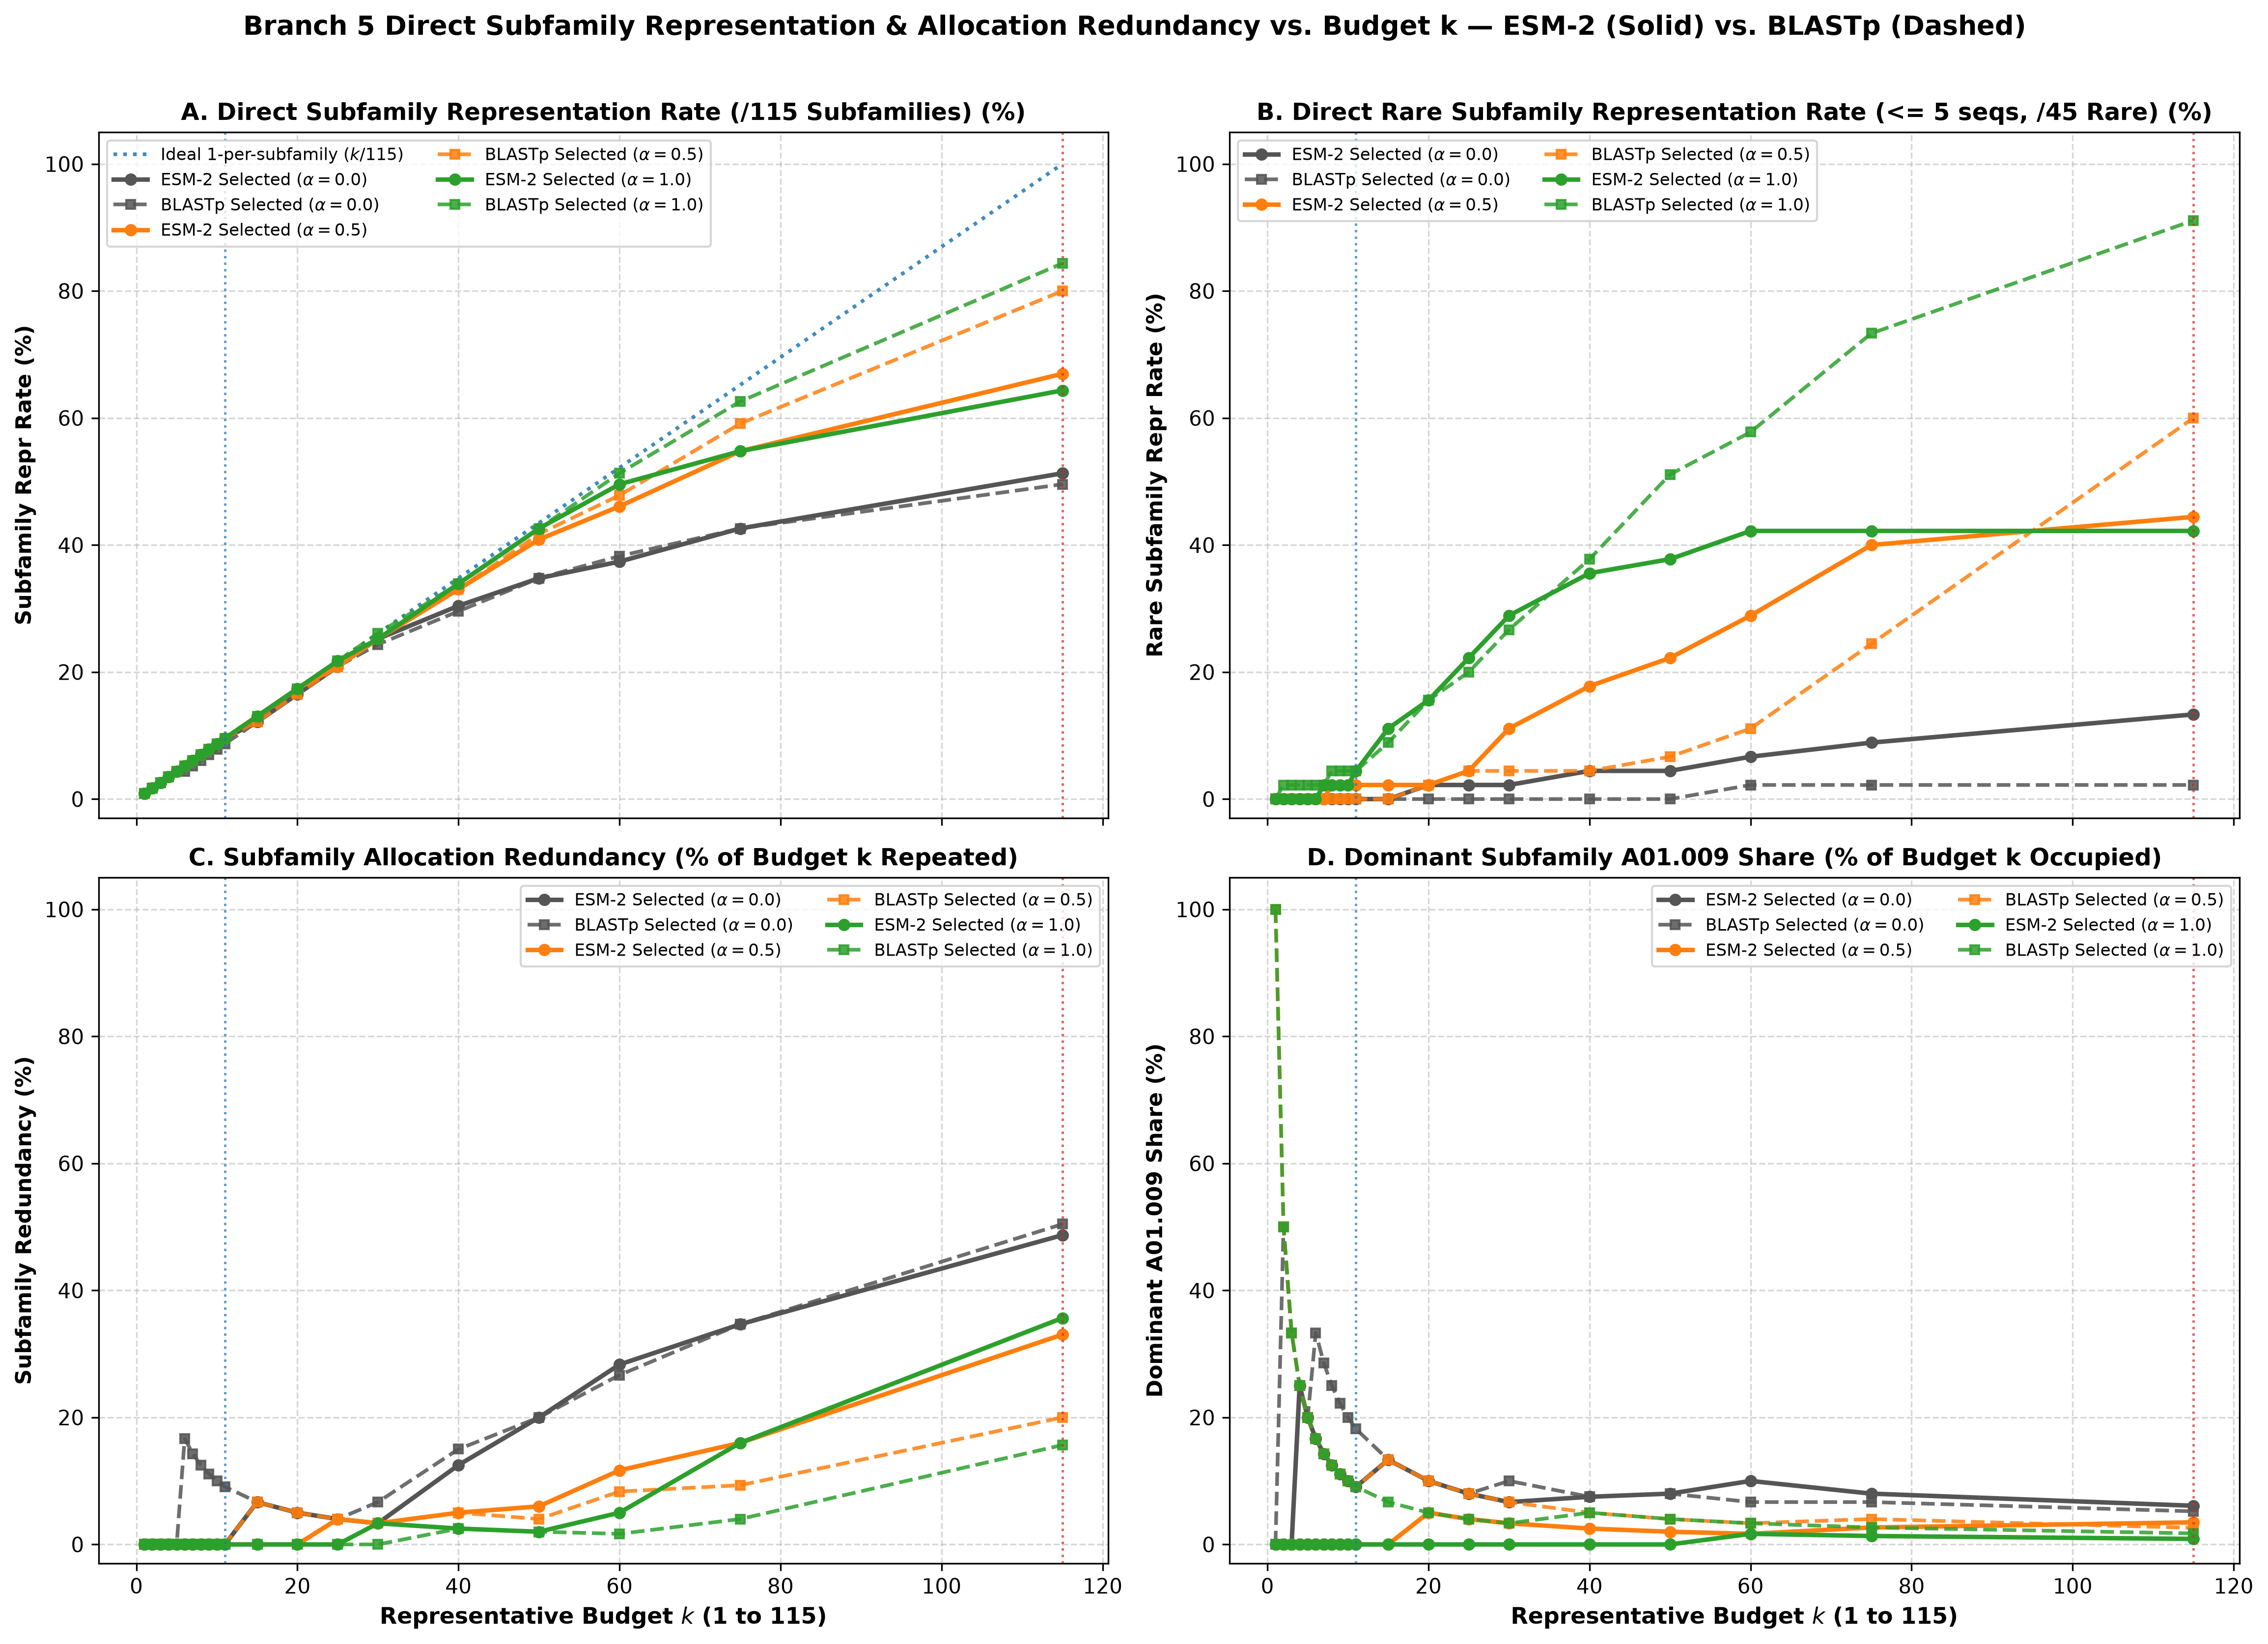
\includegraphics[width=0.92\textwidth]{Images/figures/exp5_allocation_metrics_vs_k.png}
    \caption{Sự biến thiên của bốn chỉ số cấu trúc phân bổ đại diện và tỷ lệ dư thừa theo ngân sách $k \in [1..115]$ giữa ESM-2 biểu diễn bằng đường nét liền và BLASTp biểu diễn bằng đường nét đứt qua ba mức $\alpha$.}
    \label{fig:exp5_allocation}
\end{figure}

\begin{figure}[htbp!]
    \centering
    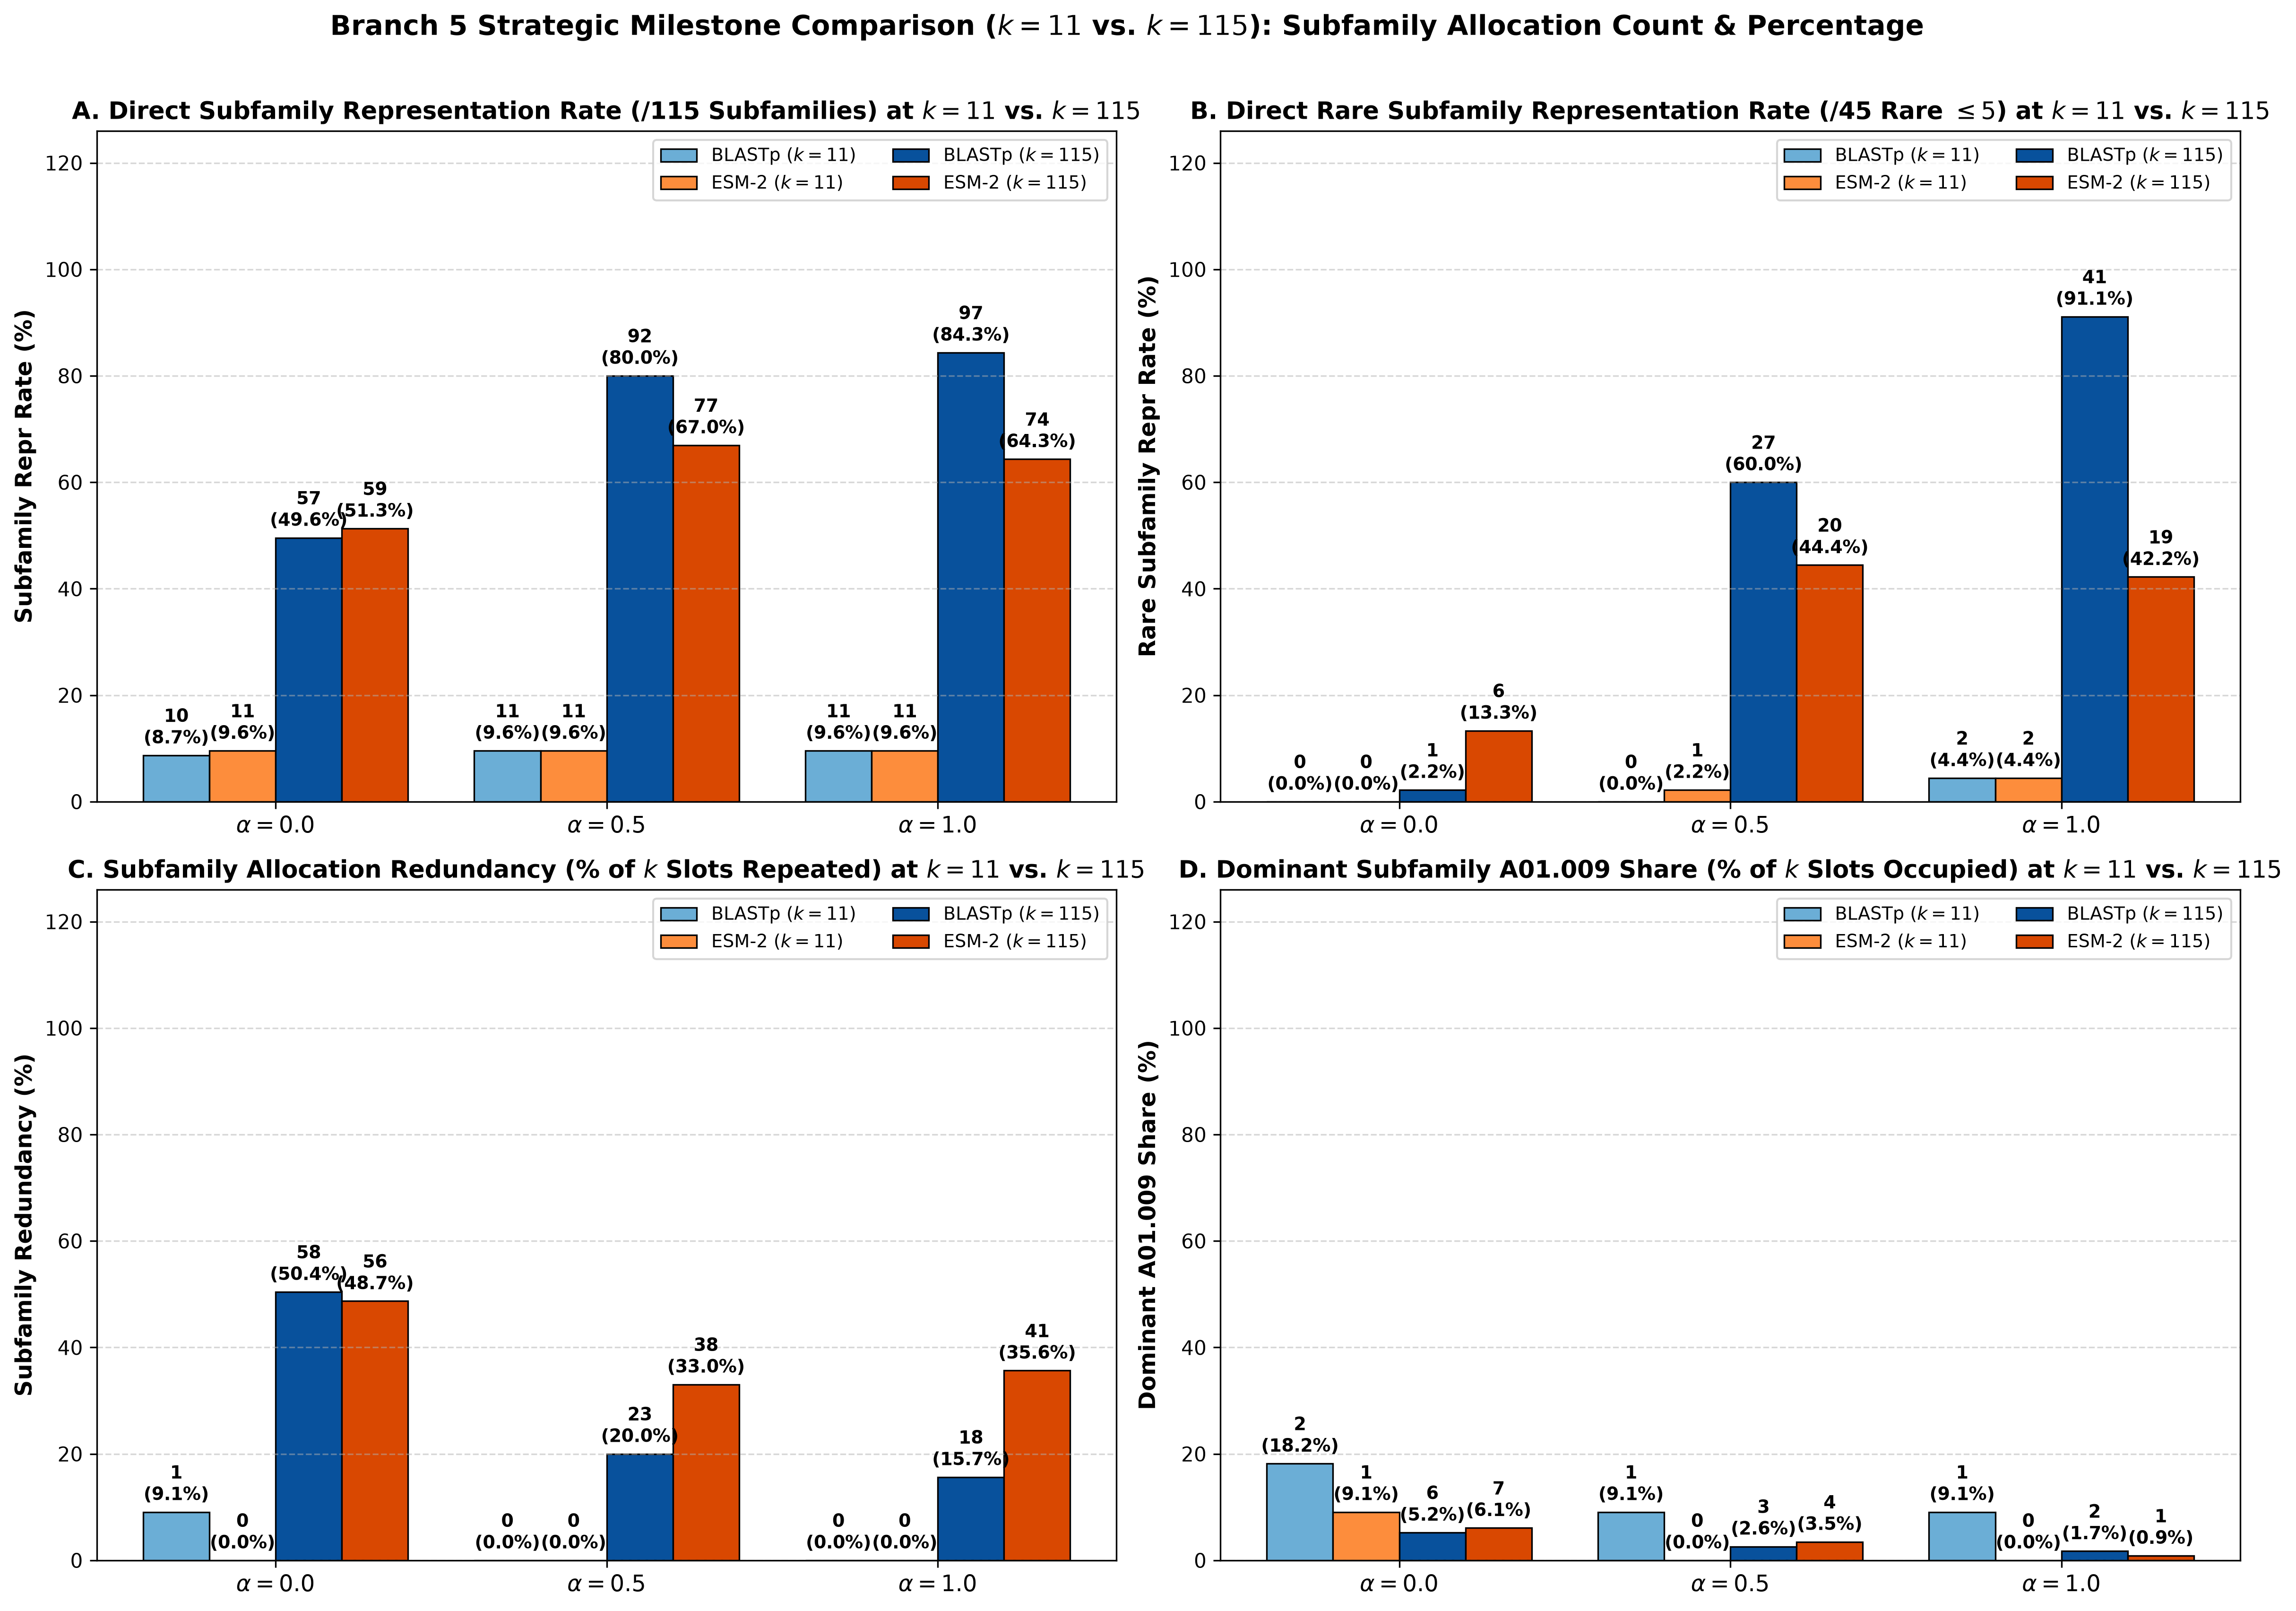
\includegraphics[width=0.92\textwidth]{Images/figures/exp5_allocation_summary_k11_k76.png}
    \caption{Biểu đồ cột ghép đối chiếu cấu trúc đại diện phân họ, đại diện nhóm hiếm, độ dư thừa và tỷ trọng đại diện của Subfamily A01.009 tại hai mốc $k = 11$ và $k = 115$.}
    \label{fig:exp5_summary}
\end{figure}

Hình~\ref{fig:exp5_allocation} và hình~\ref{fig:exp5_summary} cung cấp bằng chứng định lượng rõ ràng cho thấy phương pháp RareProtSelect hóa giải hiệu quả sự thiên lệch quy mô mẫu và tái cân bằng mức ưu tiên tối ưu hóa cho các Subfamily hiếm.

\phantomsection\label{subsec:branch6_deep_budget}

Ở các thử nghiệm trước, ngân sách tối đa được giới hạn ở ngưỡng đối chuẩn $k \le G = 115$, tương ứng tỷ lệ bình quân một đại diện trên mỗi phân họ. Tại ngưỡng này, hàm mục tiêu có trọng số $\alpha = 0{,}5$ ưu tiên ngân sách để bảo vệ các Subfamily hiếm, dẫn đến việc Subfamily lớn nhất A01.009 chỉ nhận được $3$ đại diện và chưa đạt độ bao phủ tối đa. Đối với một họ protein có độ đa dạng cao và phân tách thành nhiều phân họ với quy mô chênh lệch lớn như Family A1, ngân sách cơ sở $k = 115$ là chưa đủ để đồng thời bao phủ hết các Subfamily hiếm lẫn sự biến dị trình tự axit amin bên trong các Subfamily lớn. Do đó, thử nghiệm 6 mở rộng ngân sách lên $k_{\max} = 380$ chuỗi nhằm khảo sát quá trình hội tụ độ bao phủ của các phân họ lớn và toàn bộ siêu họ khi tăng số lượng đại diện.

Sáu mốc ngân sách chiến lược $k \in \{115, 150, 200, 270, 340, 380\}$ được thiết kế dựa trên cấu trúc phân tầng quy mô của $115$ Subfamily chính thức gồm $45$ Subfamily hiếm có $n_g \le 5$ chuỗi, $32$ Subfamily trung bình có $6 \le n_g \le 19$ chuỗi và $38$ Subfamily lớn có $n_g \ge 20$ chuỗi. Cụ thể, mốc $k = 115$ là ngưỡng ngân sách cơ sở tương ứng bình quân một đại diện cho mỗi phân họ; hai mốc $k = 150$ và $k = 200$ mở rộng thêm lần lượt $35$ và $50$ vị trí nhằm phân bổ thêm đại diện thứ hai và thứ ba cho $38$ Subfamily lớn; hai mốc $k = 270$ và $k = 340$ tăng thêm mỗi bước $70$ vị trí, tương ứng tổng số $38$ nhóm lớn và $32$ nhóm trung bình, để bổ sung đại diện thứ hai, thứ ba cho các phân họ trung bình và đại diện thứ tư, thứ năm cho các phân họ lớn; cuối cùng, mốc $k = 380$ bổ sung thêm $40$ vị trí nhằm phân bổ đại diện thứ sáu cho khối phân họ lớn, qua đó đánh giá mức độ hội tụ độ bao phủ ở vùng ngân sách cao.

Cần lưu ý một khác biệt về thiết lập tham số giữa ngưỡng ngân sách tối đa của thử nghiệm 6 và các thử nghiệm trước: tại thử nghiệm 2 và thử nghiệm 5, cơ chế xác lập thứ hạng đồng thuận qua $M = 1.000$ lần xáo trộn ngẫu nhiên độc lập được chạy với ngưỡng ngân sách tối đa $k_{\max} = 115$, ghi nhận $92$ Subfamily có đại diện và chỉ số Rare Sensitivity đạt $59{,}11\%$. Trong khi đó, tại thử nghiệm 6, quy trình đồng thuận được thiết lập trên ngưỡng ngân sách mở rộng $k_{\max} = 380$, dẫn đến sự thay đổi nhẹ về thứ tự chọn giữa các ứng viên chuỗi có độ tăng cận biên tương đương trong các lượt xáo trộn ngẫu nhiên. Vì vậy, lát cắt quan sát tại mốc $k = 115$ của cấu hình $k_{\max} = 380$ ghi nhận $88$ Subfamily có đại diện và Rare Sensitivity đạt $50{,}22\%$. Sự khác biệt này phản ánh đặc tính của cơ chế xếp hạng đồng thuận khi thay đổi số bước tích lũy $k_{\max}$, nhưng vẫn giữ nguyên xu hướng hội tụ bão hòa tổng thể.

Kết quả đo đạc thực nghiệm tại bảng~\ref{tab:exp6_milestones} cho thấy khi mở rộng ngân sách đến $k = 380$, tập đại diện trên không gian BLASTp nhận diện được chuỗi của $112$ trên $115$ Subfamily ($97{,}39\%$), trong đó có $104$ Subfamily đạt tỷ lệ nhận diện $100\%$ Sensitivity; đồng thời Subfamily lớn nhất A01.009 được phân bổ $6$ vị trí đại diện trên BLASTp và $22$ vị trí đại diện trên ESM-2, giúp độ bao phủ nội phân họ tiệm cận mức tối đa.

\begin{table}[htbp!]
\centering
\caption{Mức độ bão hòa độ bao phủ theo từng nhóm quy mô phân họ và số vị trí đại diện của Subfamily A01.009 khi mở rộng ngân sách lên $k \in [115..380]$ với $\alpha = 0{,}5$.}
\label{tab:exp6_milestones}
\vspace{4pt}
\small
\resizebox{\textwidth}{!}{%
\begin{tabular}{ccrrrrrr}
\toprule
\textbf{Không gian} & \textbf{Ngân sách $k$} & \textbf{Subfamily Representation} & \textbf{Vị trí A01.009} & \textbf{Common Sensitivity} & \textbf{Medium Sensitivity} & \textbf{Rare Sensitivity} & \textbf{Full Saturation (100\%)} \\
\midrule
BLASTp & $k = 115$ & 88 (76{,}52\%)  & 3 (2{,}61\%) & 96{,}47\% & 85{,}75\% & 50{,}22\% & 78 / 115 \\
BLASTp & $k = 150$ & 97 (84{,}35\%)  & 4 (2{,}67\%) & 99{,}13\% & 92{,}00\% & 64{,}00\% & 86 / 115 \\
BLASTp & $k = 200$ & 102 (88{,}70\%) & 4 (2{,}00\%) & 99{,}26\% & 96{,}69\% & 73{,}33\% & 93 / 115 \\
BLASTp & $k = 270$ & 107 (93{,}04\%) & 5 (1{,}85\%) & 99{,}32\% & 99{,}82\% & 82{,}22\% & 98 / 115 \\
BLASTp & $k = 340$ & 108 (93{,}91\%) & 6 (1{,}76\%) & 99{,}41\% & 100{,}00\% & 84{,}44\% & 100 / 115 \\
BLASTp & $k = 380$ & \textbf{112 (97{,}39\%)}& \textbf{6 (1{,}58\%)} & \textbf{99{,}41\%} & \textbf{100{,}00\%} & \textbf{93{,}33\%} & \textbf{104 / 115} \\
\midrule
ESM-2  & $k = 115$ & 77 (66{,}96\%)  & 4 (3{,}48\%) & 91{,}31\% & 68{,}30\% & 43{,}11\% & 69 / 115 \\
ESM-2  & $k = 150$ & 81 (70{,}43\%)  & 5 (3{,}33\%) & 94{,}00\% & 77{,}68\% & 43{,}56\% & 73 / 115 \\
ESM-2  & $k = 200$ & 82 (71{,}30\%)  & 5 (2{,}50\%) & 96{,}63\% & 77{,}68\% & 43{,}56\% & 74 / 115 \\
ESM-2  & $k = 270$ & 82 (71{,}30\%)  & 7 (2{,}59\%) & 96{,}93\% & 77{,}68\% & 43{,}56\% & 75 / 115 \\
ESM-2  & $k = 340$ & 85 (73{,}91\%)  & 21 (6{,}18\%)& 96{,}95\% & 80{,}80\% & 48{,}00\% & 79 / 115 \\
ESM-2  & $k = 380$ & \textbf{95 (82{,}61\%)} & \textbf{22 (5{,}79\%)}& \textbf{96{,}95\%} & \textbf{82{,}37\%} & \textbf{68{,}00\%} & \textbf{88 / 115} \\
\bottomrule
\end{tabular}%
}
\end{table}

Số liệu tại bảng~\ref{tab:exp6_milestones} cùng các đồ thị tại hình~\ref{fig:exp6_dominant}, hình~\ref{fig:exp6_stratified} và hình~\ref{fig:exp6_saturation} cho thấy đối với một họ protein có độ đa dạng cao và phân tách thành nhiều phân họ như Family A1, việc mở rộng ngân sách vượt ngưỡng $k = 115$ giúp giải quyết sự cạnh tranh vị trí đại diện giữa các tầng quy mô. Phân họ lớn nhất A01.009 vốn đã đạt $100{,}0\%$ Sensitivity nội phân họ ngay từ mốc ngân sách $k = 115$ với $3$ chuỗi đại diện trên BLASTp và $4$ chuỗi đại diện trên ESM-2. Khi mở rộng ngân sách lên $k = 380$, việc tăng lên $6$ chuỗi trên BLASTp và $22$ chuỗi trên ESM-2 giúp nâng cao độ bao phủ hình học ngữ nghĩa liên tục ESM của riêng phân họ này từ $91{,}88\%$ lên $93{,}67\%$ trên BLASTp và từ $93{,}27\%$ lên $95{,}81\%$ trên ESM-2. Đồng thời, thuật toán nâng tỷ lệ nhận diện của khối phân họ hiếm từ $50{,}22\%$ lên $93{,}33\%$, đưa toàn bộ $32$ Subfamily trung bình đạt bão hòa $100{,}00\%$ Sensitivity và $38$ Subfamily lớn đạt bình quân $99{,}41\%$ Sensitivity trên không gian BLASTp. Kết quả này chứng minh khi được cung cấp ngân sách mở rộng, hàm mục tiêu có trọng số $\alpha = 0{,}5$ vừa bao phủ rộng khắp các phân họ hiếm, vừa mở rộng độ bao phủ biến dị nội nhóm cho các phân họ quy mô lớn.

\begin{figure}[htbp!]
    \centering
    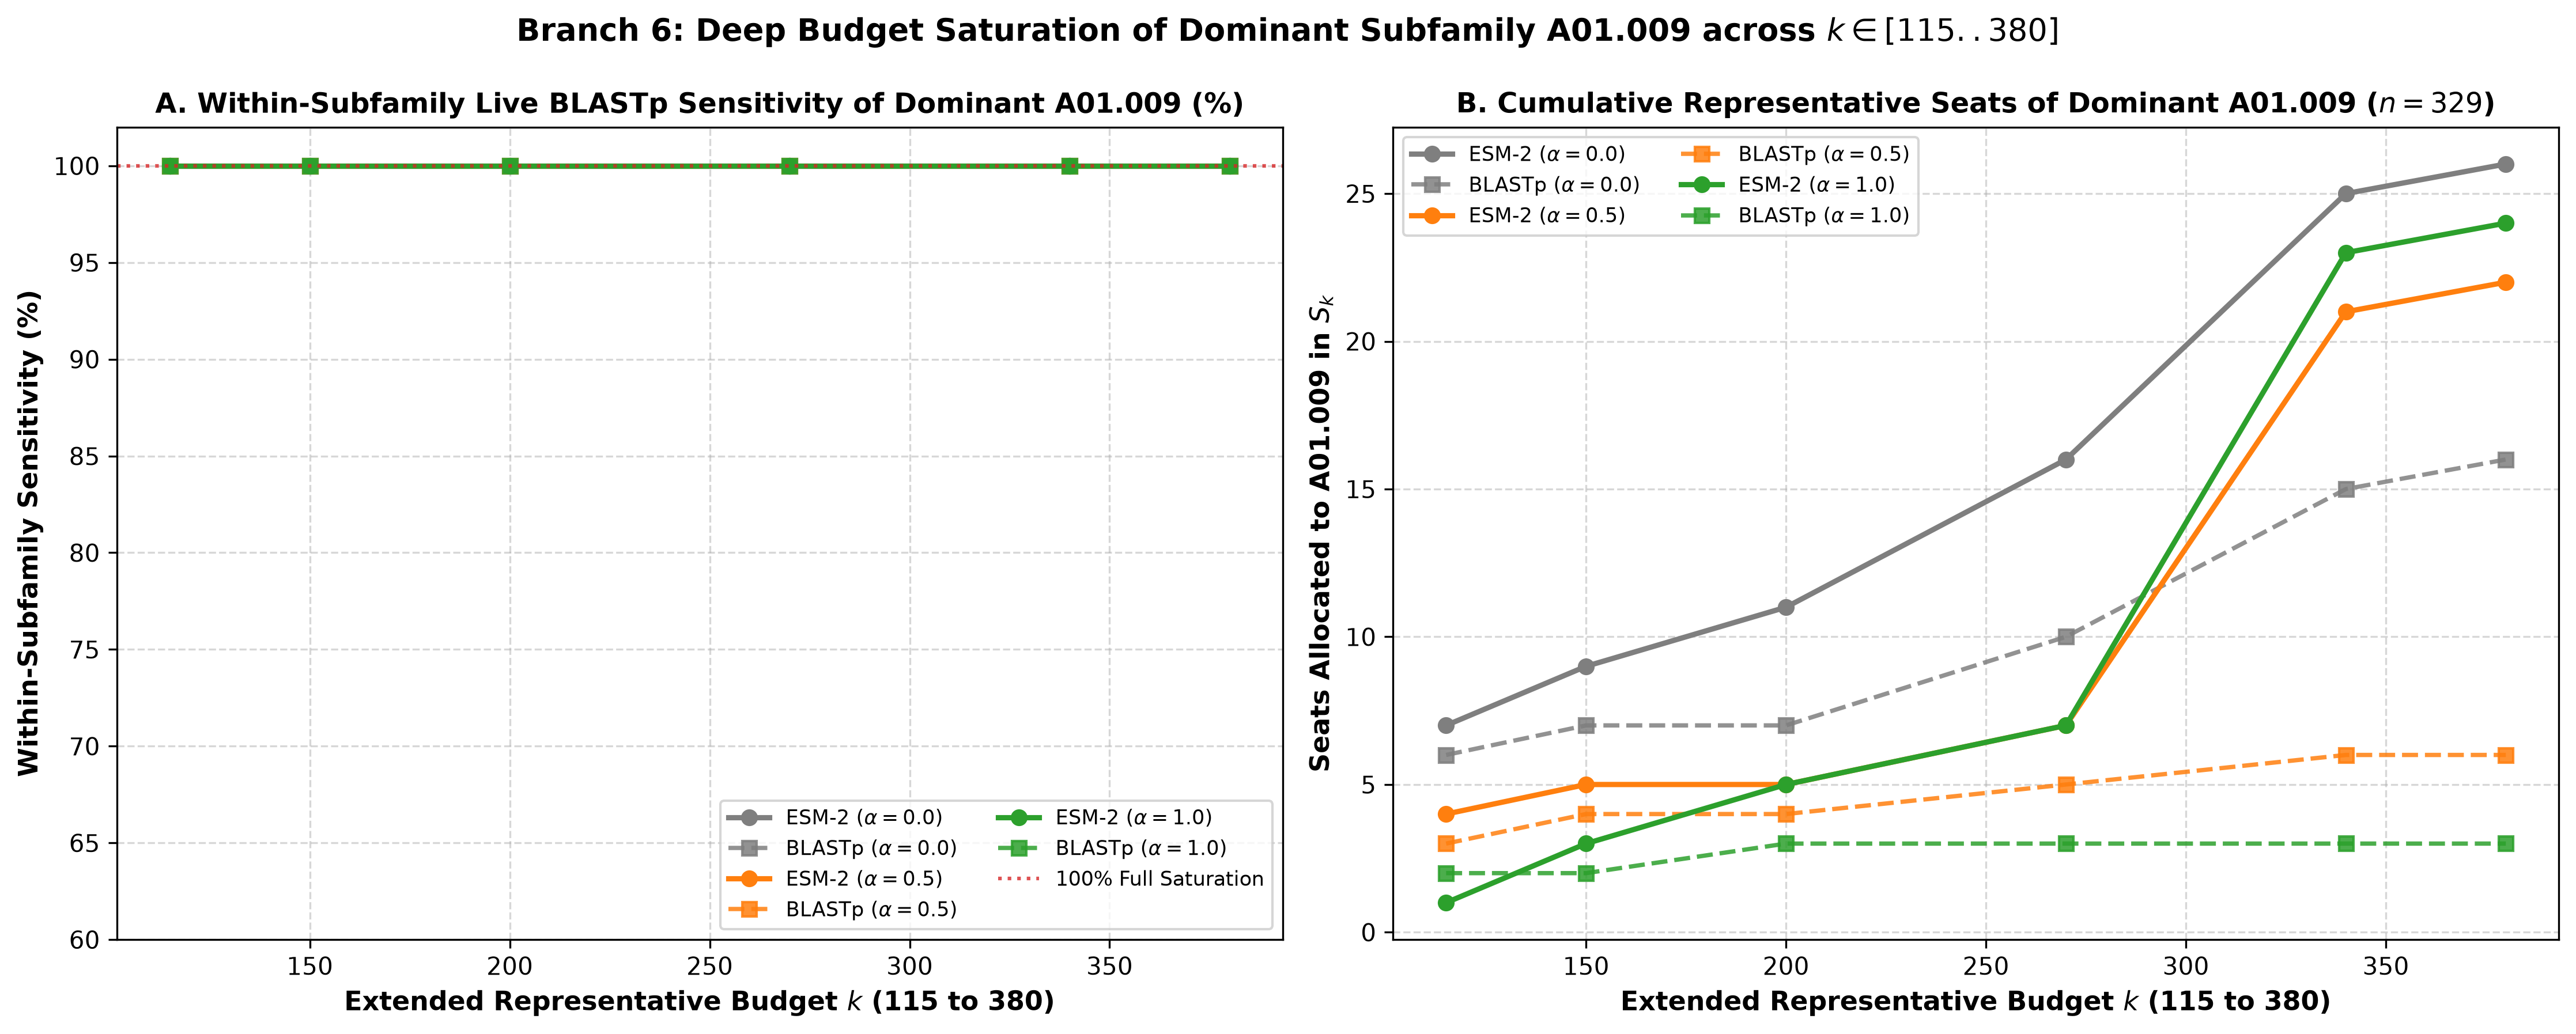
\includegraphics[width=0.92\textwidth]{Images/figures/exp6_dominant_a01_009_saturation_vs_k.png}
    \caption{Sự tích lũy số lượng đại diện và quá trình bão hòa độ bao phủ nội phân họ của Subfamily lớn nhất A01.009 khi mở rộng ngân sách lên $k \in [115..380]$.}
    \label{fig:exp6_dominant}
\end{figure}

\begin{figure}[htbp!]
    \centering
    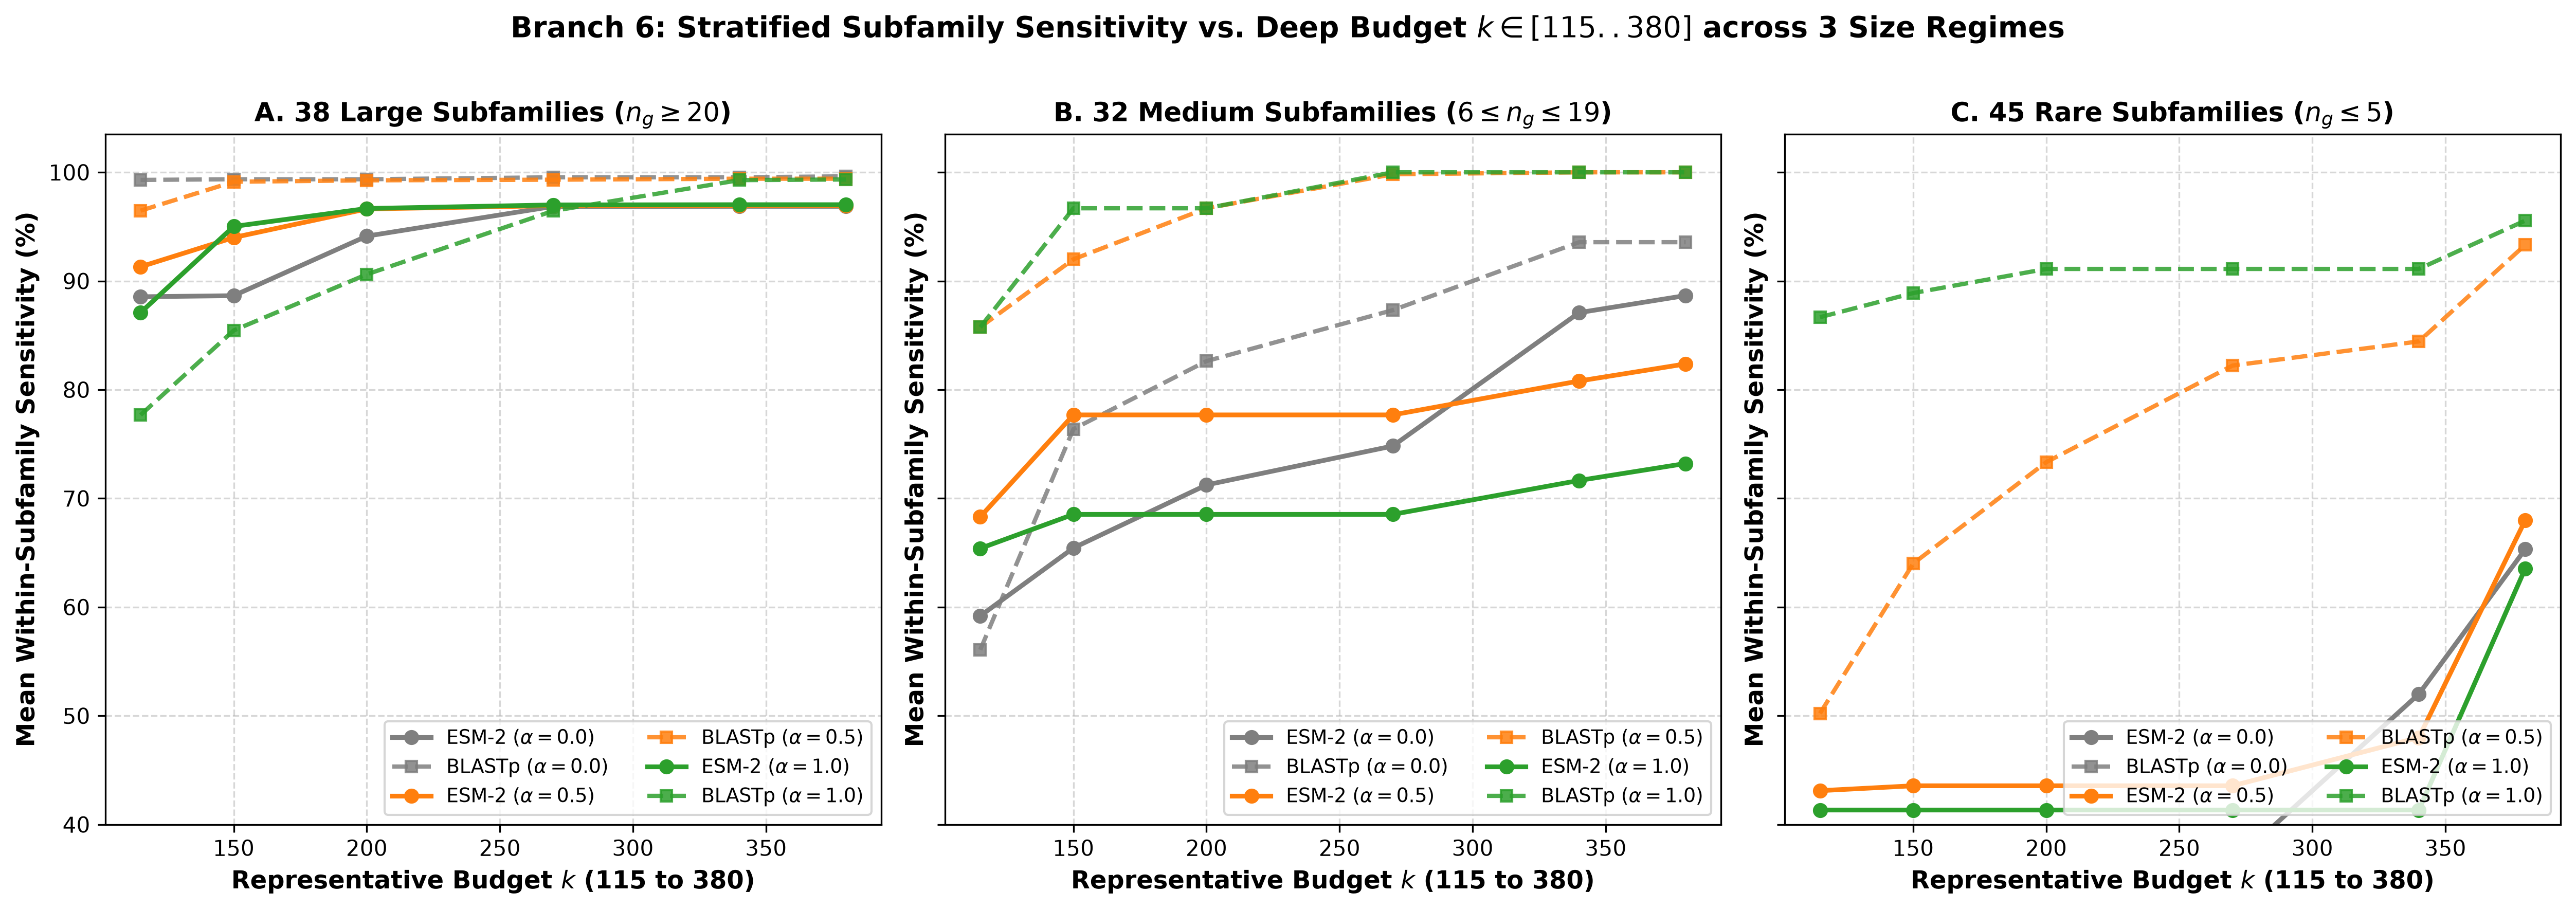
\includegraphics[width=0.92\textwidth]{Images/figures/exp6_stratified_coverage_vs_k.png}
    \caption{Xu hướng biến thiên của chỉ số Sensitivity nội phân họ phân tầng theo ba khối quy mô: lớn, trung bình và hiếm theo quy mô ngân sách mở rộng.}
    \label{fig:exp6_stratified}
\end{figure}

\begin{figure}[htbp!]
    \centering
    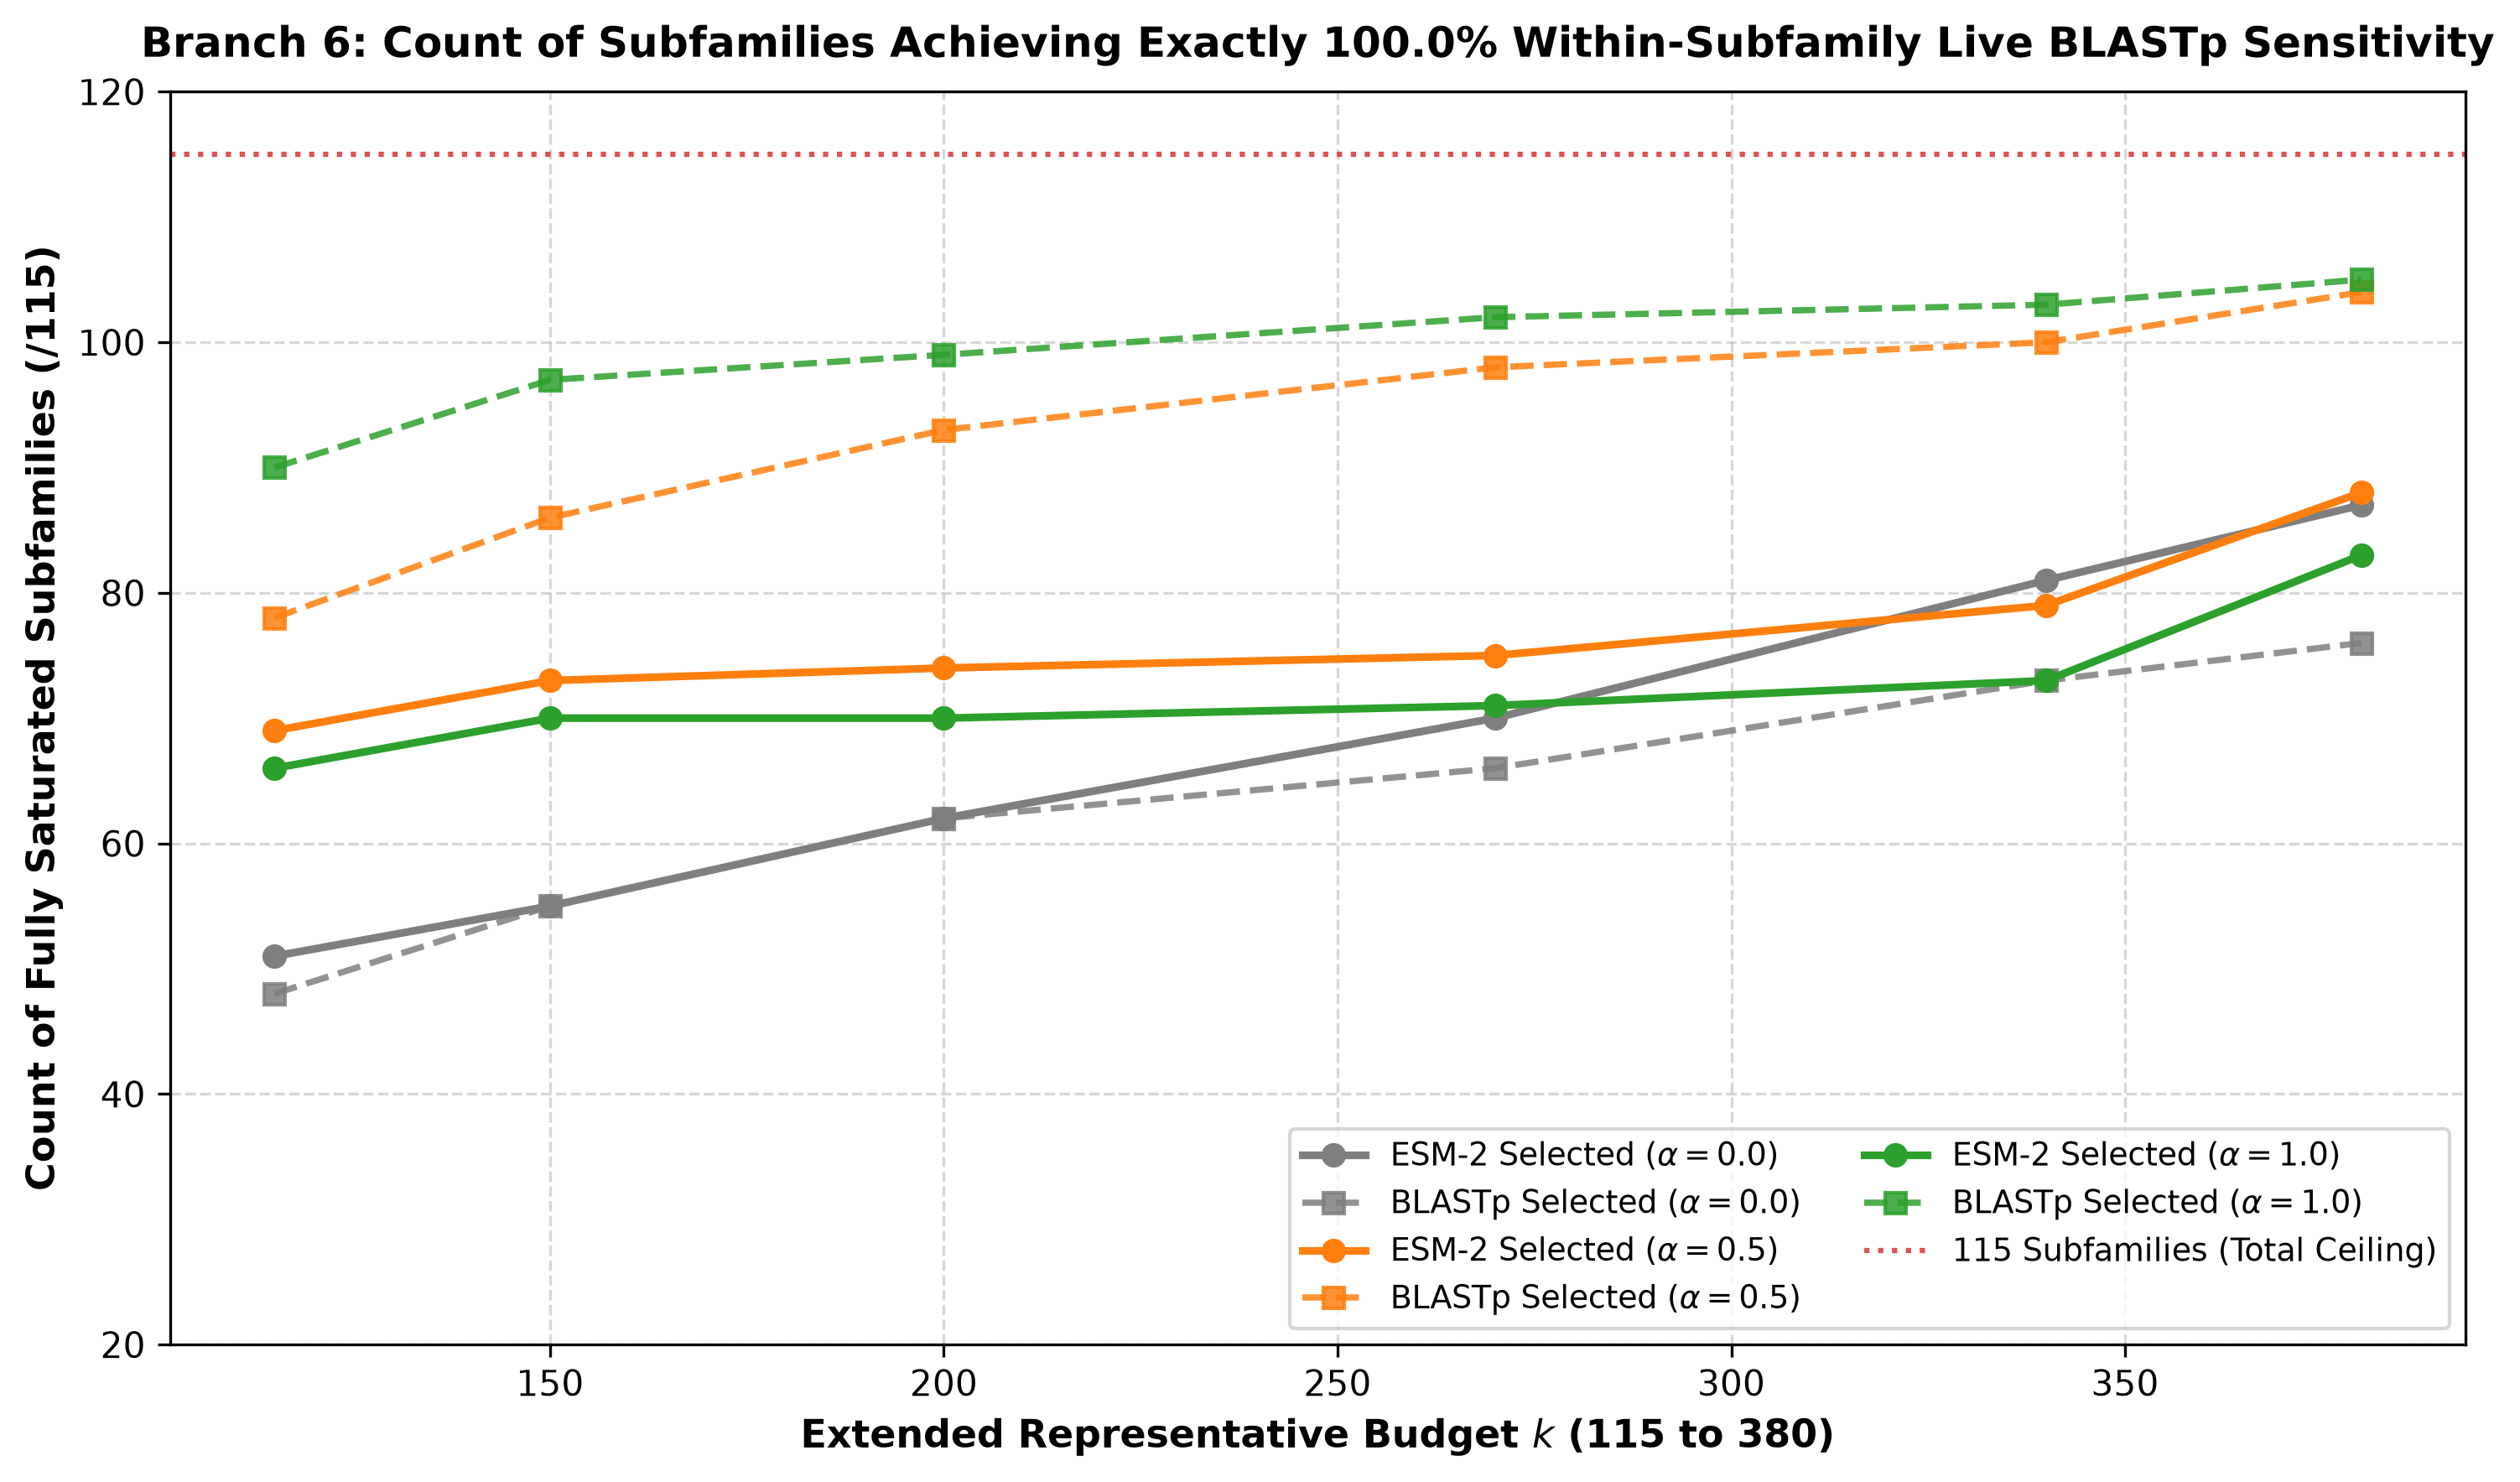
\includegraphics[width=0.82\textwidth]{Images/figures/exp6_full_saturation_count_vs_k.png}
    \caption{Số lượng Subfamily đạt bão hòa 100\% Sensitivity nội phân họ khi mở rộng ngân sách lên $k \in [115..380]$.}
    \label{fig:exp6_saturation}
\end{figure}

\FloatBarrier
\phantomsection\label{sec:exp_discussion}
\phantomsection\label{subsec:rq_resolution_matrix}

Dựa trên dữ liệu thực nghiệm xuyên suốt 6 thử nghiệm, các phát hiện khoa học và bằng chứng định lượng cốt lõi của đề tài được tổng hợp tại bảng~\ref{tab:rq_resolution}.

\begin{table}[htbp!]
\centering
\caption{Tổng hợp các phát hiện thực nghiệm và bằng chứng định lượng cốt lõi của đề tài RareProtSelect.}
\label{tab:rq_resolution}
\vspace{4pt}
\small
\begin{tabularx}{\textwidth}{L{4.2cm}Y}
\toprule
\textbf{Nội dung và thử nghiệm} & \textbf{Kết luận thực nghiệm và bằng chứng khoa học} \\
\midrule
\textbf{Hạn chế bao phủ chéo của mô hình cơ sở} \newline Thử nghiệm 1 và thử nghiệm 2 & Tạo ra sai lệch bao phủ chéo ngoài ranh giới phân họ khi đánh giá toàn cục. Tại $k=1$, chỉ số Overall Sensitivity đạt $82{,}36\%$ nhưng thực chất có tới $114$ trên $115$ Subfamily không có đại diện trực tiếp (Within-Subfamily Overall Sensitivity chỉ đạt $3{,}54\%$). Tại $k=115$, mô hình cơ sở không trọng số vẫn để sót $58$ Subfamily, tương ứng $50{,}43\%$, ở mức $0{,}0\%$ Sensitivity. \\
\addlinespace
\textbf{Tái cân bằng bằng trọng số hiếm trên BLASTp} \newline Thử nghiệm 2 & Đạt hiệu quả cao tại $\alpha = 0{,}5$: Rare Sensitivity tăng gấp $26{,}6$ lần từ $2{,}22\%$ lên $59{,}11\%$, Macro-Average Sensitivity tăng $+29{,}59\%$, khôi phục tính đại diện cho $35$ Subfamily trong khi Overall Sensitivity không giảm, đạt $94{,}13\%$. \\
\addlinespace
\textbf{Mở rộng không gian ngữ nghĩa liên tục ESM-2} \newline Thử nghiệm 3 & Bảo tồn cụm ngữ nghĩa liên tục. Trên ma trận tương đồng đã dịch tâm với $\beta=0{,}70$, trọng số $\alpha=0{,}5$ tăng Rare Coverage ESM gấp $3{,}4$ lần, từ $12{,}85\%$ lên $43{,}21\%$, bắt đầu lựa chọn được đại diện của nhóm hiếm sớm ngay từ mốc $k=8$. \\
\addlinespace
\textbf{Kiểm chứng chéo hai chiều giữa hai không gian} \newline Thử nghiệm 4 & Làm rõ sự đảo chiều về hiệu năng theo ngân sách $k$: ESM-2 đạt kết quả cao hơn gấp từ $1{,}6$ lần đến $4{,}0$ lần ở dải ngân sách từ $k = 8$ đến $k = 75$, trong khi BLASTp đạt kết quả cao hơn tại $k=115$ do tính cô lập phân họ của ma trận thưa. \\
\addlinespace
\textbf{Cơ chế phân bổ vị trí đại diện trong tập nghiệm} \newline Thử nghiệm 5 & Hóa giải sự thiên lệch quy mô mẫu. Tỷ lệ dư thừa giảm từ $50{,}43\%$ xuống $20{,}00\%$, số vị trí đại diện của A01.009 tại $k=115$ được kiểm soát từ $6$ xuống $3$, chiếm $2{,}61\%$ ngân sách, phân bổ đại diện cho $92$ trên $115$ Subfamily và $27$ trên $45$ nhóm hiếm. \\
\addlinespace
\textbf{Hội tụ độ bao phủ khi mở rộng ngân sách} \newline Thử nghiệm 6 & Khi mở rộng ngân sách lên $k = 380$ với $\alpha = 0{,}5$, không gian BLASTp nhận diện chuỗi của $112$ trên $115$ Subfamily ($97{,}39\%$) với $104$ Subfamily đạt $100\%$ Sensitivity; Subfamily lớn nhất A01.009 được tăng cường từ $3$ lên $6$ chuỗi trên BLASTp (nâng Coverage ESM từ $91{,}88\%$ lên $93{,}67\%$) và từ $4$ lên $22$ chuỗi trên ESM-2 (nâng Coverage ESM từ $93{,}27\%$ lên $95{,}81\%$), duy trì $100{,}0\%$ Live BLASTp Sensitivity và chứng minh khả năng vừa bảo toàn nhóm hiếm vừa mở rộng độ bao phủ ngữ nghĩa cho các phân họ lớn có biến dị nội nhóm rộng. \\
\bottomrule
\end{tabularx}
\end{table}

Bảng~\ref{tab:rq_resolution} tổng hợp các phát hiện thực nghiệm chính, làm rõ ba đóng góp phương pháp luận của đề tài: thứ nhất, làm rõ cơ chế sai lệch bao phủ chéo ngoài ranh giới phân họ của mô hình không trọng số; thứ hai, thiết lập cấu hình trọng số cân bằng với mức tăng trưởng gấp $26{,}6$ lần về chỉ số Rare Sensitivity trên không gian BLASTp và gấp $3{,}4$ lần trên không gian ESM-2; và thứ ba, xác lập quy luật phân bổ đại diện công bằng, giảm độ dư thừa từ $50{,}43\%$ xuống $20{,}00\%$ và chuyển dịch vị trí đại diện sang các Subfamily hiếm.

\phantomsection\label{subsec:method_comparison}

So với các công cụ gom cụm và chọn đại diện truyền thống như CD-HIT~\cite{cdhit} hay MMseqs2~\cite{mmseqs2}, RareProtSelect thể hiện ba ưu điểm về phương pháp luận: thứ nhất, khả năng kiểm soát trực tiếp lực lượng tập đại diện theo bài toán ràng buộc ngân sách $|S| \le k$ thay vì phụ thuộc vào việc dò tìm ngưỡng tương đồng cứng dựa trên phương pháp heuristic; thứ hai, bảo đảm toán học giải tích chặt chẽ qua cận xấp xỉ Nemhauser $(1 - 1/e) \approx 63{,}2\%$ giá trị tối ưu toàn cục mà các thuật toán gom cụm heuristic không thể cung cấp; và thứ ba, cơ chế tái cân bằng trọng số linh hoạt qua tham số $\alpha$, cho phép người dùng chủ động điều tiết mức độ ưu tiên bảo tồn nhóm hiếm và tối ưu hóa hiệu quả đánh đổi đa mục tiêu trên các phân bố sinh học mất cân bằng lớn về quy mô. Kết quả thực nghiệm khẳng định tính hiệu quả của khung phương pháp đề xuất.
